\documentclass{article}

\usepackage{url}
\usepackage[hmargin=1.5in]{geometry}
\usepackage{enumitem}
\usepackage{amsmath}
\usepackage{amssymb}
\usepackage{amsthm}
\usepackage{eqnarray}
\usepackage{graphicx}
\usepackage[svgnames]{xcolor} %% for revisions
\usepackage{xparse} %% for squiggly underlines
\usepackage{tikz-cd} %% for term norm scratch work
\usepackage{tikz}

% TikZ libraries
\usetikzlibrary{bbox}
\usetikzlibrary{fadings}

% hat tip TeX.SE user Andrew Stacey
%   https://tex.stackexchange.com/a/82503/6934
%   https://tex.stackexchange.com/questions/82425/tikz-radial-shading-of-a-ring#comment176908_82503
\pgfdeclareradialshading{radialedge}{\pgfpointorigin}{%
  color(0bp)=(transparent!0);
  color(20bp)=(transparent!0);
  color(22bp)=(transparent!10);
  color(24bp)=(transparent!90);
  color(25bp)=(transparent!100)
}
\pgfdeclarefading{radial edge}{\pgfuseshading{radialedge}}%

\setcounter{tocdepth}{2}

%%\theoremstyle{definition}
\newtheorem{defn}{Definition}
\theoremstyle{plain}
\newtheorem{prop}{Proposition}
\newtheorem{lemma}{Lemma}
\newtheorem{thm}{Theorem}
\newtheorem{rmk}{Remark}
\newtheorem{cor}{Corollary}

% list formatting
\newlist{conditions}{itemize}{1}
\setlist[conditions]{leftmargin=24mm, rightmargin=12mm}
\makeatletter
% hat tip TeX.SE user31729
%   https://tex.stackexchange.com/a/328393/6934
\newcommand{\cond}[1]{\item[(\textsc{#1})]\protected@edef\@currentlabel{\textsc{#1}}}
\newcommand{\condconst}[2]{\item[($\text{\textsc{#1}} \mid #2$)]\protected@edef\@currentlabel{$\text{\textsc{#1}} \mid #2$}}
\makeatother

% convenience aliases
\newcommand{\maps}{\colon}

% group action
\newcommand{\acts}{\mathbin{\raisebox{\depth}{\rotatebox{-90}{$\circlearrowright$}}}}

% symbology
\newcommand{\Z}{\mathbb{Z}}
\newcommand{\R}{\mathbb{R}}
\newcommand{\C}{\mathbb{C}}
\let\Re\relax
\DeclareMathOperator{\Re}{Re}
\newcommand{\laplace}{\mathcal{L}}
\newcommand{\series}[1]{\tilde{#1}}
\newcommand{\fracderiv}[3]{\partial^{#1}_{#2, #3}}

% function spaces
\newcommand{\cont}{\mathcal{C}}
\newcommand{\holo}{\mathcal{H}}
\newcommand{\singexp}[2]{\mathcal{H}L^\infty_{#1, #2}}
\newcommand{\singexpalg}[1]{\singexp{#1}{\bullet}}
\newcommand{\holoL}[1]{\mathcal{H}L^{#1}} %% may no longer be needed
\newcommand{\expHoloL}[2]{\mathcal{H}L^{#1}_{#2}} %% may no longer be needed

% operator under consideration
\newcommand{\volterra}{\mathcal{V}}
\newcommand{\hardpart}{\mathcal{V}_0}
\newcommand{\softpart}{\mathcal{V}_\star}
\newcommand{\kerwhole}{k}
\newcommand{\hardker}{k_0}
\newcommand{\softker}{k_\star}
\newcommand{\solwhole}{f}
\newcommand{\solproto}{f_0}
\newcommand{\solptb}{f_\star}

% domain
\newcommand{\domain}{\Omega}
\newcommand{\near}{\Omega_\text{near}}
\newcommand{\far}{\Omega_\text{far}}

% drafting environments
\newenvironment{verify}{\color{ForestGreen}}{\color{black}}
\newenvironment{brainstorm}{\color{violet}\begin{itemize}}{\end{itemize}\color{black}}

\title{Regular singular Volterra equations on complex domains}
\author{Veronica Fantini and Aaron Fenyes}
\date{}

\begin{document}
\maketitle

\begin{abstract}
The inverse Laplace transform can turn a linear differential equation on a complex domain into an equivalent Volterra integral equation on a real domain. This can make things simpler: for example, a differential equation with irregular singularities can become a Volterra equation with regular singularities. It can also reveal hidden structure, especially when the Volterra equation extends to a complex domain.

Our main result is to show that for a certain kind of regular singular Volterra equation on a complex domain, there is always a unique solution of a certain form. As a motivating example, this kind of Volterra equation arises when using Laplace transform methods to solve a {\em level~1} differential equation.
\end{abstract}

\tableofcontents

\begin{brainstorm}
\item \textcolor{gray}{\textit{(Aaron)} State Lemma~\ref{lem:perturbed_volterra} just the way we want it.}
\begin{itemize}
    \item \textcolor{gray}{Proofread and drop old version.}
\end{itemize}
\item \textcolor{gray}{\textit{(Aaron)} Finish introduction}
\begin{itemize}
\item \textcolor{gray}{\textit{(Veronica)} Brainstorm: what are we trying to say in this paper? Write ideas in the to-do list at the bottom of the motivation section.}
\item \textcolor{gray}{\textit{(Veronica)} Revise introduction, if desired.}
\end{itemize}
\color{gray}
\item \textit{(Veronica)} Say in Section~\ref{setting:perturbed} that $\volterra = \hardpart + \softpart$ and write arguments we need for bounds on whole kernel (for example, in Equation~\ref{near-limit}.
\color{gray}
\item \textit{(Veronica)} Review old blue text in Section~\ref{setting:perturbed} and decide whether we want to keep any of it. Can drop unilaterally. 
\color{violet}
\item Revise stuff related to proof of main results.
\begin{itemize}
        \item \textcolor{gray}{\textit{(Aaron)} Add proof of Lemma~\ref{lem:perturbed_volterra} to Section~\ref{sec:existence and uniqueness}}
        \item \textcolor{gray}{\textit{(Aaron)} Revise proof of Theorem~\ref{thm:general_volterra} in Section~\ref{sec:existence and uniqueness}}
        \begin{itemize}
            \item \textcolor{gray}{Proofread revised proof.}
        \end{itemize}
        \item \textit{(Aaron)} State the desired result of Section~\ref{sec:image under soft_part}.
        \color{gray}
        \item \textit{(Veronica)} Add motivation to Section~\ref{sec:image under soft_part}, explaining that the desired result of the section follows from a more general result about the smoothing effect of $\softpart$ (Proposition~\ref{prop:smoothing}). \textcolor{green}{I added a Corollary to explicitly write how Proposition \ref{prop:smoothing} implies the regularity we want for $\softpart f_0$}
        \color{violet}
        \item \textbf{(Aaron)} Confirm again that removed $\tau+\gamma$ upper bound on $\rho$ was unnecessary.
\end{itemize}
\item \textcolor{gray}{Revise text around main results.}
\begin{itemize}
    \item \textcolor{gray}{Decide whether to keep Lemma~\ref{lem:perturbed_volterra} as a lemma, or to make it a theorem, and make Theorem~\ref{thm:general_volterra} its corollary. Change order as appropriate.} \textcolor{purple}{Keep Lemma~\ref{lem:perturbed_volterra} as a lemma. State it after Theorem~\ref{thm:general_volterra}.}
    \color{gray}
    \item \textit{(Veronica)} Convert ``proof'' blocks to plain prose after main results. 
\end{itemize}
\color{gray}
\item \textbf{(Veronica)} Edit statement of Theorem~\ref{thm:example} 
\begin{itemize}
    \item Edit or remove statements about making $\Lambda$ big enough
    \item Figure out how to clean up $Q(-\zeta')$ business
\end{itemize}
\color{violet}
\item \textcolor{gray}{Start finalizing notation for the two parts of the operator and the two parts of the solution.}
\begin{itemize}
    \item \textcolor{gray}{Choose subscripts or decorations to tell things apart in equations.} \textcolor{gray}{Change $\hardpart$ with $\volterra_0$ and $\softpart$ with $\volterra_\star$. Same for $\hardker$ and $\softker$.}
    \item \textcolor{gray}{Choose names to tell things apart in prose. Currently using ``prototypical operator,'' ``prototype solution.'' Come up with names for perturbation stuff.}
\end{itemize}
\item \textbf{(Aaron)} Read through Section~\ref{sec:example}.
\color{gray}
\item \textbf{(Veronica)} Consider revising notation for roots. 
\begin{itemize}
\item ``$P$ is a monic degree-$d$ polynomial with only simple zeros;''
\item ``$Q$ is a degree-$(d-1)$ polynomial, and $Q(-\alpha) \neq 0$ for for every zero $-\alpha$ of $P$;''---or even say it without formulas.
\end{itemize}
\color{violet}
\item \textcolor{gray}{\textbf{(Aaron)} Change list formatting so that extra indentation applies only to conditions. We're using the \texttt{enumitem} package.}
\item Work on acknowledgements
\begin{itemize}
\item \textbf{(Aaron)} Add people Aaron had conversations with
\item \textbf{(Aaron)} Think about rephrasing FMHJ acknowledgement (ERC one can't be changed).
\end{itemize}
\item \textcolor{gray}{Reconsider using $\lesssim$ (but still leaning not to)}
\begin{itemize}
    \item \textcolor{gray}{\textbf{(Aaron)} As an example, show how we could rewrite the argument in proof of Proposition~\ref{prop:asymptotic at infinity} with $\lesssim$.}
\end{itemize}
\item \textcolor{gray}{Write abstract.}
\item \textcolor{gray}{\textbf{(Veronica)} Add table of contents.}
\item \textcolor{gray}{Replace $\psi_0$ with $\chi$.}
\item \textcolor{gray}{Replace $\epsilon$ with $\gamma$.}
\item \textbf{(Aaron)} Use hyperref package. (For link color, use the same green as the verify environment, or maybe turquoise or RoyalBlue?)
\end{brainstorm}
\section{Introduction}
\subsection{Motivation}\label{motivation}
In its most basic form, the Laplace transform $\laplace$ turns exponential-type functions of a real ``position'' variable $\zeta$ into holomorphic\begin{verify}\footnote{\begin{verify}Suppose the magnitude of the Laplace transform integrand is Riemann-integrable on $(0, \infty)$. Write $z$ in terms of its real and imaginary parts as $x + iy$. Since the integrand is holomorphic with respect to $z$, the operator $\frac{\partial}{\partial\overline{z}} = \frac{1}{2}\left(\frac{\partial}{\partial x} + i\frac{\partial}{\partial x}\right)$ annihilates it. Using the comparison version of Leibniz's rule for improper integrals (Theorem~11.10 of A First Course in Real Analysis, by Protter and Morrey) with $\frac{\partial}{\partial x}$ and $\frac{\partial}{\partial y}$, we see that $\frac{\partial}{\partial\overline{z}}$ annihilates the whole integral.\end{verify}}\end{verify} functions of a complex ``frequency'' variable $z$. Through identities like
\begin{align*}
\frac{\partial}{\partial z} \laplace \varphi & = \laplace(z\varphi) \\
\laplace k\;\laplace \varphi & = \laplace(k * \varphi) \\
z^{-\lambda} \laplace \varphi & = \laplace\,\partial^{-\lambda} \varphi,
\end{align*}
where $\partial^{-\lambda}$ is the Riemann-Liouville fractional integral of order $\lambda \in (0, \infty)$, the Laplace transform pulls differential operators on the frequency domain back to Volterra integral operators on the position domain. The favorable regularity properties and comprehensive theory of Volterra equations can thus be brought to bear on linear differential equations.

Some differential equations pull back to Volterra equations with real-analytic kernels, which extend to holomorphic Volterra equations on complex extensions of the position domain. Solutions that look unrelated in the frequency domain may turn out to be linked by analytic continuation along the complex position domain, as seen in the phenomenon of {\em resurgence} \cite{EcalleIII}\cite{lectures-marino}\cite[Section 2.4]{sternin1995borel}.

Differential equations with irregular singularities in the frequency domain can pull back to Volterra equations with regular singularities in the position domain. In Section~\ref{sec:example}, we'll see this helpful behavior in the class of differential equations that Ecalle calls {\em level~1}, which includes classical examples like the modified Bessel equation, the equations describing the vibration modes of beams that taper in certain ways \textcolor{orange}{[find citation]}, and the Airy equation after a change of coordinate. This last example generalizes to some level 1 equations that feature in current research, like the Airy-Lucas and higher Airy equations~\cite[Equations 3.2 and 3.8]{charbonnier22}\cite{durugo_higher}.

From our experience with solving level~1 differential equations by Borel summation, we expect each of the corresponding integral equations to have a special kind of solution when the integration base point coincides with a regular singularity. Let's say we've chosen the position variable $\zeta$ so that the integration base point is at $\zeta = 0$, and our position-domain Volterra operator has a holomorphic kernel $k(a, a')$ with a $\tau/\zeta(a)$ singularity. Assuming the residue $\tau$ is real and positive, we expect to find a solution with the following features:
\begin{itemize}
\item It has an $O\big(\zeta^{\tau-1}\big)$ singularity at $\zeta = 0$.
\item It's of exponential type, meaning that it's $O\big(e^{\Lambda|\zeta|}\big)$ for some $\Lambda \in \R$ as $\zeta$ grows.
\end{itemize}
These conditions are just strong enough to ensure that the solution has a well-defined Laplace transform, which by construction will satisfy the differential equation we started with in the frequency domain. The first condition also tells us that the Laplace-transformed solution is $O(z^{-\tau})$ as the frequency variable $z$ grows.

Our goal is to justify the expectations above with an existence and uniqueness result, stated in Section~\ref{sec:results}. We'll achieve it by embodying our expectations in a Banach space of holomorphic functions---the space $\singexp{\tau-1}{\Lambda}(\domain)$ defined in Section~\ref{fn-spaces}. We'll apply our results to level $1$ differential equations in Section~\ref{sec:example}.
\subsection{Notation for uniform bounds}
Given a complex-valued function $\varphi$ and a non-negative, real-valued function $\omega$, we'll write $\varphi \lesssim \omega$ to say that $|\varphi|$ is bounded by a constant multiple of $\omega$. Unless we say otherwise, the bound holds throughout the domain where both functions are defined.
\subsection{Setting}\label{setting}
\subsubsection{The domain}\label{setting:domain}
Throughout this paper, as described in Section~\ref{motivation}, the position variable $\zeta$ will be the standard coordinate on $\C$. Take a simply connected open set $\domain \subset \C$ that touches but doesn't contain $\zeta = 0$. We also assume:
\begin{conditions}
\cond{star}\label{cond:star} The set $\domain$ is star-shaped around $\zeta = 0$. In other words, for any $a \in \domain$, a straight path from $\zeta = 0$ to $a$ stays in $\domain$. Since $\domain$ doesn't contain $\zeta = 0$, we'll always leave that starting point out of the path.
\end{conditions}
For the applications we have in mind, $\domain$ might look something like the set pictured below, which satisfies Condition~\eqref{cond:star}.
\begin{center}
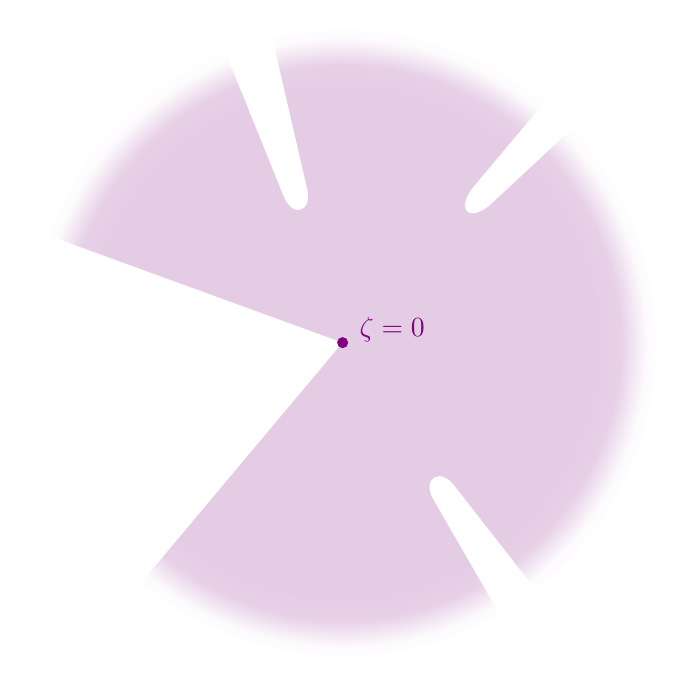
\begin{tikzpicture}
\newcommand{\spill}{4}
\fill[violet!20, bezier bounding box, path fading=radial edge]
  (-\spill, -\spill) (\spill, \spill)
  (0, 0) -- (160:\spill)
  arc (160:112:\spill) -- (112:2) .. controls (112:1.7) and (103:1.7) .. (103:2) -- (103:\spill)
  arc (103:50:\spill) -- (50:2.6) .. controls (50:2.2) and (43:2.2) .. (43:2.6) -- (43:\spill)
  arc (43:-52:\spill) -- (-52:2.3) .. controls (-52:2) and (-60:2) .. (-60:2.3) -- (-60:\spill)
  arc (-60:-130:\spill) -- (0, 0);
\fill[violet] circle (0.7mm) node[anchor=195, outer sep=1mm] {$\zeta = 0$};
\end{tikzpicture}
\end{center}
\subsubsection{The prototype operator}\label{setting:basic}
The prototypical example of the kind of operator we'll be working with is a holomorphic Volterra operator $\hardpart$ with a separable kernel and a regular singularity at $\zeta = 0$.

Being a holomorphic Volterra operator means that $\hardpart$ sends each holomorphic function $\varphi$ on $\domain$ to a new holomorphic function
\[ [\hardpart\,\varphi](a) = \int_{\zeta = 0}^a \hardker(a, \cdot)\,\varphi\;d\zeta. \]
Being separable means that the kernel $\hardker(a, a')$ factors into a function of $a$ times a function of $a'$. We'll suppose this product can be written as a ratio
\[ \hardker(a, a') = - \frac{q(a')}{p(a)}, \]
where $p$ and $q$ are holomorphic functions on $\domain$. Having a regular singularity at $\zeta = 0$ means the following:
\begin{conditions}
\condconst{sing}{\tau}\label{cond:sing} For some non-zero constant $\tau$---the {\em residue} of the singularity---the difference
\[ \hardker(a, a') - \frac{\tau}{\zeta(a)} \]
is bounded on a neighborhood of $\big(\zeta(a), \zeta(a')\big) = (0, 0)$ in $\domain^2$.
\end{conditions}
We'll assume that $\tau$ is real and positive.

Our definition of a regular singularity implies that as $|\zeta|$ goes to zero, $|p|$ also goes to zero, while $|q|$ settles into a compact interval that doesn't include zero.
\begin{verify}
[\textit{Proof.} Fix any $a'$ in the neighborhood where the difference above is bounded. By confining $a$ to small enough neighborhoods of $\zeta = 0$, we can make $|\tau/\zeta(a)|$ arbitrarily large, forcing $|q(a')/p(a)|$ to become arbitrarily large to satisfy the definition. Since $a'$ is fixed, the only way for this ratio to get arbitrarily large is for $|p(a)|$ to get arbitrarily small.]
\end{verify}
For some of our results, we'll also need to control $|p|$ and $|q|$ in various ways as $|\zeta|$ goes to infinity.
\begin{conditions}
\condconst{slow}{\lambda_0}\label{cond:slow} We can find constants $\lambda_p$ and $\lambda_\text{ratio}$ with
\begin{align*}
\left|\frac{1}{p}\right| & \lesssim e^{\lambda_p |\zeta|} &
\left|\frac{q}{p}\right| & \le \lambda_\text{ratio}
\end{align*}
outside some neighborhood of $\zeta = 0$ in $\domain$. In addition, $|1/p|$ and $|q/p|$ are bounded outside every neighborhood of $\zeta = 0$ in $\domain$; the bound may depend on the neighborhood. Note that this only constrains the ratio of $p$ and $q$ when they're evaluated at the same point. The constants will only enter our reasoning through their sum, $\lambda_0 = \lambda_p + \lambda_\text{ratio}$.
\end{conditions}
This condition explains why $\domain$ might have the sort of shape illustrated in Section~\ref{setting:domain}. As $\domain$ stretches out toward infinity, it has to part around the zeros of $p$, keeping well away from every zero except the one at $\zeta = 0$.
\begin{conditions}
\condconst{diag$_0$}{\lambda_\Delta}\label{cond:diag-basic} We can find a constant $\lambda_\Delta$ with
\[ \big| \hardker(a, a') \big| \lesssim e^{\lambda_\Delta|\zeta(a)-\zeta(a')|} \]
over all $a$ in $\domain$ outside some neighborhood of $\zeta = 0$, and all $a' \in \domain$.
%%outside a neighborhood of $\zeta(a) = 0$ in $\domain^2$.
\end{conditions}
We'll occasionally mention an optional condition on $p$ that allows us to state our main results more explicitly.
\begin{conditions}
\condconst{reg-p}{B, \epsilon}\label{cond:reg-p}
For some non-zero constant $B$ and some $\epsilon > 0$,
\[ p \in B\zeta + O\big(|\zeta|^{1 + \epsilon}\big) \]
at $\zeta = 0$.
\end{conditions}
\subsubsection{The perturbed operator}\label{setting:perturbed}

Now, let's perturb $\hardpart$ to a more general operator $\volterra=\hardpart +\softpart$. The perturbation $\softpart$ doesn't have a separable kernel,\footnote{Unless $\softpart$ is zero, of course.} but does have a smoothing effect that counteracts the singularity of $\hardpart$ (as we'll show in Proposition \ref{prop:smoothing}). To get the smoothing effect, we'll require the kernel $\softker$ of $\softpart$ to vanish to some order $\gamma > 0$ on the diagonal in $\Omega^2$. This requirement, combined with two others, will be made precise in Condition~\eqref{cond:eps-lambda}.

Since $\softpart$ is a holomorphic Volterra operator, $\softker$ is a holomorphic function on $\domain^2$. We'll allow $\softker(a, a')$ to have a simple pole at $\zeta(a) = 0$, like $\hardker(a, a')$ does, but we won't allow any sharper singularity. We'll also put an exponential bound on how fast $\softker$ grows away from the diagonal, mimicking Condition~\eqref{cond:diag-basic} on $\hardker$. Altogether, we'll require:
\begin{conditions}
\condconst{diag$_\star$}{\gamma, \lambda_\Delta}\label{cond:eps-lambda} For some constant $\gamma > 0$, we have
\[ \big| \softker(a, a') \big| \lesssim\frac{|\zeta(a)-\zeta(a')|^\gamma}{|\zeta(a)|}\,e^{\lambda_\Delta|\zeta(a)-\zeta(a')|}\]
over all $a, a' \in \domain$.
\end{conditions}
Notice that this condition prevents $\softker$ from being separable---unless it's zero, of course.

Like $\hardker$, the combined kernel $k = \hardker + \softker$ of $\volterra$ grows in a controlled way when its arguments are near $\zeta = 0$, and when the difference between its arguments grows. We'll provide specific bounds in Section~\ref{sec:bounds on k}. 

\subsection{Main results}\label{sec:results}
We want to show that when $\volterra$ is a regular singular Volterra operator of the kind described in Section~\ref{setting:perturbed}, the equation $f = \volterra f$ has a unique solution of a certain form. For the prototypical operator $\hardpart$ described in Section~\ref{setting:basic}, this solution can be written explicitly.
\begin{thm}\label{thm:basic_volterra}
Suppose $\hardpart$ satisfies {\em Condition \eqref{cond:sing}}. Then the equation
\[ f = \hardpart f \]
has the {\em prototype solution}
\begin{equation}\label{eqn:test_solution}
\solproto(a) = \frac{1}{p(a)} \exp\left(-\int_{b}^{a}\frac{q}{p}\;d\zeta\right).
\end{equation}
Changing the base point $b \in \domain$ just multiplies $f_0$ by a non-zero constant.
\end{thm}
We'll prove this result in Section~\ref{sec:construction}.

The solution $\solproto$ from Theorem~\ref{thm:basic_volterra} has, at worst, a mild power-law singularity at $\zeta = 0$. With stronger constraints on $\hardpart$, we can also ensure that $\solproto$ grows at most exponentially as $|\zeta| \to \infty$. The function spaces defined in Section~\ref{fn-spaces} express both of these regularity properties.
\begin{thm}\label{thm:proto-growth}
Suppose $\hardpart$ satisfies {\em Condition~\eqref{cond:sing}}. Then, on a small enough neighborhood of $\zeta = 0$, we have $|\solproto| \lesssim |\zeta|^{\tau-1}$.

Suppose $\hardpart$ also satisfies {\em Condition~\eqref{cond:slow}}. Then $f_0$ belongs to the space $\singexp{\tau-1}{\lambda_0}(\domain)$ defined in Section~\ref{fn-spaces}.
\end{thm}
We'll prove this result in Section~\ref{sec:asymptotics}.

\begin{rmk}
Under stronger conditions on $p$, we can get a better estimate of the prototype solution near $\zeta = 0$, as described in Proposition~\ref{prop:better-proto-estimate} from Section~\ref{sec:asymptotics} for details.

%%Suppose $p$ falls into the class $B\zeta + O\big(|\zeta|^2\big)$, for some constant $B$, when it's restricted to some neighborhood of $\zeta = 0$.

%%for some constant $B$, we can strengthen the conclusion of Theorem~\ref{thm:proto-growth}. Under {\em Condition~\eqref{cond:sing}}, we can show that $\solproto \in B\zeta^{\tau-1} + O(|\zeta|^\tau)$.

%%If $q$ has a limit at $\zeta = 0$, the solution $f_0$ from Theorem~\ref{thm:basic_volterra} can be written as a constant multiple of $\zeta^{\tau-1}$ plus a function which is $O(\zeta^\tau)$ at $\zeta = 0$.
\end{rmk}
\color{black}

%%---------
%%Once we've understood the prototype solution $\solproto$, we can deform it to a solution of the equation we originaly set out to solve---the one involving the perturbed operator $\volterra = \hardpart + \softpart$ from Section~\ref{setting:perturbed}.

%%The prototype solution $\solproto$ will be our reference point for studying the perturbed operator $\volterra = \hardpart + \softpart$ from Section~\ref{setting:perturbed}.

%%Once we've understood the prototypical operator $\hardpart$, we perturb it to the more general operator $\volterra = \hardpart + \softpart$ described in Section~\ref{setting:perturbed}. The prototypical

%%Since $\hardpart$ is the regular singular part of the perturbed operator $\volterra = \hardpart + \softpart$ from Section~\ref{setting:perturbed},
%%---------
When we perturb $\hardpart$ to the more general operator $\volterra = \hardpart + \softpart$ from Section~\ref{setting:perturbed}, the equation we're trying to solve gets more complicated, but its regular singularity at $\zeta = 0$ stays essentially the same. We might therefore expect to find a solution that looks like $\solproto$ near the singularity, differing only by a less singular perturbation. If we strengthen the constraints on $\hardpart$ a little more, this expectation is fulfilled.
\begin{thm}\label{thm:general_volterra}
Suppose $\hardpart$ satisfies {\em Conditions \eqref{cond:sing}}, \eqref{cond:slow}, and \eqref{cond:diag-basic}, and $\softpart$ satisfies {\em Condition~\eqref{cond:eps-lambda}}. Then the equation
\[f = \volterra f\]
has a unique solution $f$ in the affine subspace
\[ f_0 + \singexpalg{\tau-1+\gamma}(\Omega) \]
of the space $\singexpalg{\tau-1}(\Omega)$ defined in Section~\ref{fn-spaces}. Here, $f_0$ is the prototype solution \eqref{eqn:test_solution} from Theorems \ref{thm:basic_volterra}--\ref{thm:proto-growth}, which belongs to the space $\singexp{\tau-1}{\lambda_0}(\Omega)$.

For any $\rho > \tau$, the uniqueness of the solution still holds in $f_0 + \singexpalg{\rho-1}(\Omega)$. In other words, lowering $\rho$ into $(\tau, \tau+\gamma)$ to allow a sharper singularity won't reveal any more solutions, and raising $\rho$ too high to admit the solution found in $f_0 + \singexpalg{\tau-1+\gamma}(\Omega)$ will leave no solution at all.
\end{thm}
This result will follow from a more general result about inhomogeneous equations.
\begin{lemma}\label{lem:perturbed_volterra}
Suppose $\hardpart$ satisfies {\em Conditions \eqref{cond:sing}} and \eqref{cond:diag-basic}, and $\softpart$ satisfies {\em Condition \eqref{cond:eps-lambda}}. Suppose we're also given a function $g$, which for some $\rho > \tau$ belongs to the space $\singexpalg{\rho-1}(\Omega)$ defined in Section~\ref{fn-spaces}. Then the inhomogeneous equation
\[ f = \volterra f + g, \]
has a unique solution $f$ in the space $\singexpalg{\rho-1}(\Omega)$.
\end{lemma}
We'll prove Lemma~\ref{lem:perturbed_volterra} in Sections \ref{sec:V is a contraction}--\ref{sec:existence and uniqueness}, using the contraction mapping theorem. The heart of the argument is Proposition~\ref{prop:get-contraction}, which shows us how to find relevant subspaces where $\volterra$ is a contraction.

We'll reduce Theorem~\ref{thm:general_volterra} to Lemma~\ref{lem:perturbed_volterra} in Section~\ref{sec:existence and uniqueness}, by rewriting the homogeneous equation we want to solve as an inhomogeneous equation in a more regular space. To show that the inhomogeneous term, $\softpart f_0$, is regular enough, we'll use Proposition~\ref{prop:smoothing} from Section~\ref{sec:image under soft_part} to show that $\softpart$ improves on the regularity of $f_0$ described by Theorem~\ref{thm:proto-growth}.

\begin{rmk}
Under stronger conditions on $p$, Theorem~\ref{thm:general_volterra} can be restated to provide a unique solution in the affine subspace
\[ \zeta^{\tau-1} + \singexpalg{\tau-1+\gamma}(\Omega). \]
as described in Proposition~\ref{prop:alt-general_volterra} from Section~\ref{sec:existence and uniqueness}.
\end{rmk}
%%To prove Theorem~\ref{thm:general_volterra}, we will rewrite the homogeneous equation we want to solve as an inhomogeneous one, with $\softpart f_0$ as the inhomogeneous term.

%%We will reduce Theorem~\ref{thm:general_volterra} to Lemma~\ref{lem:perturbed_volterra} in Section~\ref{sec:existence and uniqueness}, with the help of Proposition~\ref{prop:smoothing} from Section~\ref{sec:image under soft_part}, which can be used to show that $\softpart f_0$ is regular enough to serve as the inhomogeneous term in the lemma.
\subsection{Acknowledgements}

This paper is a result of the ERC-SyG project, Recursive and Exact New Quantum Theory (ReNewQuantum) which received funding from the European Research Council (ERC) under the European Union's Horizon 2020 research and innovation programme under grant agreement No 810573. 

We thank Fondation Mathematique Jacques Hadamard for supporting the visit of the second author at IH\'ES, under the program \textit{Junior Scientific Visibility}.
\begin{brainstorm}
\item Kihyun Kim and his visitor (possibly Prof. Soonsik Kwon or Sung-Jin Oh)
\item Angeliki Menegaki
\end{brainstorm}
\section{Function spaces for holomorphic Volterra operators}\label{fn-spaces}
\subsection{Weighted holomorphic $L^\infty$ spaces}\label{sec:fn-space-defs}
Throughout this paper, as described in Section~\ref{motivation}, the ``position'' variable $\zeta$ will be the standard coordinate on $\C$. Take a simply connected open set $\Omega \subset \C$ that touches but doesn't contain $\zeta = 0$. Let $\cont(\Omega)$ be the space of continuous complex-valued functions on $\Omega$. Give $\cont(\Omega)$ the compact-open topology, recalling that this is the coarsest topology in which the seminorm $f \mapsto \sup_K |f|$ is continuous for every compact subset $K \subset \Omega$~\cite[Example~2.6 and \S 4 notes]{fnl-cpx-anal}. The holomorphic functions form a closed subspace $\holo(\Omega) \subset \cont(\Omega)$~\cite[Proposition~3.14]{fnl-cpx-anal}.

Fixing a real constant $\Lambda$, let's restrict our attention to holomorphic functions on $\Omega$ which are bounded by constant multiples of $e^{\Lambda|\zeta|}$. One might describe these functions as being uniformly of exponential type $\Lambda$.\footnote{Recall that a function is of exponential type $\Lambda$ if for every $\varepsilon>0$ there is a constant $A_\varepsilon$ (which depends on $\varepsilon$) such that $|f(x)|\leq A_\varepsilon e^{(\Lambda+\varepsilon)|x|}$. We instead require that there exists a uniform constant $A$ such that for every $\varepsilon>0$ the bound holds.} They form a space $\singexp{0}{\Lambda}(\Omega)$, which we'll equip with the norm $\|f\|_{0,\Lambda} = \sup_\Omega e^{-\Lambda|\zeta|}\,|f|$. With respect to the seminorm on $\holo(\Omega)$ given by a compact set $K \subset \Omega$, the inclusion map $\singexp{0}{\Lambda}(\Omega) \hookrightarrow \holo(\Omega)$ has norm $\sup_K e^{\Lambda |\zeta|}$. That means the inclusion is continuous.
\begin{prop}\label{exp-complete}
The space $\singexp{0}{\Lambda}(\Omega)$ is complete.
\end{prop}
\begin{proof}
Take a Cauchy sequence $f_1, f_2, f_3, \ldots \in \singexp{0}{\Lambda}(\Omega)$. The inclusion map $\singexp{0}{\Lambda}(\Omega) \hookrightarrow \holo(\Omega)$ is bounded with respect to each of the seminorms on $\holo(\Omega)$ given by $|f| \mapsto \sup_K |f|$ for compact subsets $K \subset \Omega$, so our sequence is Cauchy in $\holo(\Omega)$ too. Since $\holo(\Omega)$ is complete~\cite[Proposition~3.5]{fnl-cpx-anal},\footnote{That is, a sequence which is Cauchy in each of the seminorms on $\holo(\Omega)$ will always converge in the topology of $\holo(\Omega)$, which is the coarsest topology in which all of the seminorms are continuous.} our sequence converges to a function $f$ there.

The Cauchy property in $\singexp{0}{\Lambda}(\Omega)$ tells us that for any $r > 0$, we can find some $n$ for which $e^{-\Lambda |\zeta|}\,|f_k - f_n| \le r$ whenever $k \ge n$. Since convergence in $\holo(\Omega)$ implies pointwise convergence, we can see as $k$ grows that $e^{-\Lambda |\zeta|}\,|f - f_n| \le r$. This shows that our sequence converges to $f$ in the norm $\|\cdot\|_{0,\Lambda}$. We can also see from this argument that $f$ is in $\singexp{0}{\Lambda}$: picking some $r > 0$, we observe that
\begin{align*}
e^{-\Lambda |\zeta|}\,|f| & \le e^{-\Lambda |\zeta|}\,|f - f_n| + e^{-\Lambda |\zeta|}\,|f_n| \\
& \le r + \|f_n\|_{0,\Lambda}
\end{align*}
for the corresponding $n$, showing that $e^{-\Lambda |\zeta|}\,|f|$ is bounded.
\end{proof}

Now, let's relax our norm to allow both exponential growth at infinity and a power-law singularity at $\zeta = 0$. Let $\singexp{\sigma}{\Lambda}(\Omega)$ be the space of holomorphic functions on $\Omega$ which are bounded by constant multiples of $|\zeta|^\sigma e^{\Lambda|\zeta|}$. Give it the norm $\|f\|_{\sigma,\Lambda} = \sup_\Omega |\zeta|^{-\sigma} e^{-\Lambda|\zeta|}\,|f|$. Reprising the arguments from above, we can show that the inclusion $\singexp{\sigma}{\Lambda}(\Omega) \hookrightarrow \holo(\Omega)$ is continuous, and we can generalize Proposition~\ref{exp-complete}:
\begin{prop}
The space $\singexp{\sigma}{\Lambda}(\Omega)$ is complete.
\end{prop}
\subsection{Continuous inclusions between different $\singexp{\sigma}{\Lambda}(\Omega)$}\label{sec:inclusions}
\begin{prop}\label{prop:inclus-ge-exp}
If $\Lambda'\leq\Lambda$, the inclusion map $\singexp{\sigma}{\Lambda'}(\Omega)\hookrightarrow \singexp{\sigma}{\Lambda}(\Omega)$ is continuous.
\end{prop}
\begin{proof}
By definition,
\[ \|f\|_{\sigma,\Lambda}=\sup_{\Omega} |\zeta|^{-\sigma}\,e^{-\Lambda |\zeta|}\, |f|. \]
The norm $\|\cdot\|_{\sigma, \Lambda'}$ is designed to give $|f| \le |\zeta|^\sigma\,e^{\Lambda'|\zeta|}\,\|f\|_{\sigma, \Lambda'}$, which tells us that
\begin{align*}
\|f\|_{\sigma,\Lambda} & \leq \sup_{\Omega} |\zeta|^{-\sigma}\,e^{-\Lambda |\zeta|}\,|\zeta|^\sigma\,e^{\Lambda'|\zeta|}\,\|f\|_{\sigma, \Lambda'}\\
&=\sup_{\Omega} e^{-(\Lambda-\Lambda') |\zeta|}\,\|f\|_{\sigma, \Lambda'}\\
&\leq \|f\|_{\sigma,\Lambda'}.
\end{align*}
In the last step, we use the assumption that $\Lambda' \le \Lambda$.
\end{proof}
As we mentioned in Section~\ref{sec:fn-space-defs}, one might describe $\singexp{0}{\Lambda}(\domain)$ as the space of functions on $\domain$ which are uniformly of exponential type $\Lambda$. Taking the union of these spaces over all $\Lambda \in \R$, we get the space $\singexpalg{0}(\domain)$ that contains all functions of exponential type. Having continuous inclusions between the subspaces $\singexp{0}{\Lambda}(\domain)$ as $\Lambda$ increases, we can give $\singexpalg{0}(\domain)$ a meaningful topology: the finest topology that makes all the inclusions $\singexp{0}{\Lambda}(\domain) \hookrightarrow \singexpalg{0}(\domain)$ continuous.\footnote{In category-theoretic language, $\singexpalg{0}(\domain)$ is the limit of the family $\singexp{0}{\Lambda}(\domain)$.}
\begin{prop}\label{prop:inclus-lt-pow-gt-exp}
If $\sigma'>\sigma$ and $\Lambda'<\Lambda$, the inclusion map $\singexp{\sigma'}{\Lambda'}(\Omega)\hookrightarrow \singexp{\sigma}{\Lambda}(\Omega)$ is continuous.
\end{prop}
\begin{proof}
By definition,
\begin{align*}
\|f\|_{\sigma,\Lambda}&=\sup_{\Omega} |\zeta|^{-\sigma}  e^{-\Lambda |\zeta|} |f|\\
&= \sup_{\Omega} |\zeta|^{\sigma'-\sigma}\,|\zeta|^{-\sigma'}\,e^{-\Lambda'|\zeta|}\,  e^{-(\Lambda-\Lambda') |\zeta|} \, |f|.
\end{align*}
The function $|\zeta|^{\sigma'-\sigma}\,  e^{-(\Lambda-\Lambda') |\zeta|}$ is bounded near $\zeta = 0$ because the power of $|\zeta|$ is positive, and it's bounded far from $\zeta = 0$ thanks to the decaying exponential. Hence,
\begin{align*}
\|f\|_{\sigma,\Lambda}&\leq C\sup_\Omega  |\zeta|^{-\sigma'}\, e^{-\Lambda'|\zeta|} \, |f|\\
&=C \|f\|_{\sigma',\Lambda'}
\end{align*}
for $C = \sup_{\Omega}  |\zeta|^{\sigma'-\sigma}\,  e^{-(\Lambda-\Lambda') |\zeta|}$.
\end{proof}
\begin{prop}\label{prop:inclus-lt-pow-alg}
When $\sigma' > \sigma$, there's a continuous inclusion $\singexpalg{\sigma'}(\Omega)\hookrightarrow \singexpalg{\sigma}(\Omega)$.
\end{prop}
\begin{proof}
For each $\Lambda'$, we can get a continuous inclusion $\singexp{\sigma'}{\Lambda'}(\Omega) \hookrightarrow \singexpalg{\sigma}(\Omega)$ by choosing some $\Lambda > \Lambda'$ and composing the continuous inclusion $\singexp{\sigma'}{\Lambda'}(\Omega) \hookrightarrow \singexp{\sigma}{\Lambda}(\Omega)$ given by Proposition~\ref{prop:inclus-lt-pow-gt-exp} with the continuous inclusion $\singexp{\sigma}{\Lambda}(\Omega) \hookrightarrow \singexpalg{\sigma}(\Omega)$ that we get by definition. For any $\Lambda'' < \Lambda'$, the inclusions $\singexp{\sigma'}{\Lambda''}(\Omega) \hookrightarrow \singexpalg{\sigma}(\Omega)$ and $\singexp{\sigma'}{\Lambda'}(\Omega) \hookrightarrow \singexpalg{\sigma}(\Omega)$ constructed above automatically commute with the inclusion $\singexp{\sigma'}{\Lambda''}(\Omega) \hookrightarrow \singexp{\sigma'}{\Lambda'}(\Omega)$ given by Proposition~\ref{prop:inclus-ge-exp}, because we're ultimately working in the vector space of holomorphic functions on $\Omega$. Because of how the topology on $\singexpalg{\sigma'}(\Omega)$ is defined, this gives us the desired continuous inclusion $\singexpalg{\sigma'}(\Omega)\hookrightarrow \singexpalg{\sigma}(\Omega)$.
\end{proof}
\section{Solving holomorphic Volterra equations}
\subsection{Overview}
The results stated in Section~\ref{sec:results} lay out a method for solving the regular singular Volterra equation $\solwhole = \volterra \solwhole$. We'll now show that the method works by proving those results.

We start by constructing the prototype solution $\solproto$ from the kernel of $\hardpart$, which is the separable operator that gives $\volterra = \hardpart + \softpart$ its regular singularity. We'll show in Section~\ref{sec:proto-construction-regularity} that $\solproto$ satisfies the equation $\solproto = \hardpart \solproto$ and belongs to the space $\singexp{\tau-1}{\lambda_0}(\domain)$.

To see what the perturbation $\softpart$ does to $\solproto$, we'll show in Section~\ref{sec:image under soft_part} that $\softpart$ has a smoothing effect, reducing the sharpness of any power-law singularity at $\zeta = 0$. In particular, it sends $\solproto$ into $\singexpalg{\tau-1+\gamma}(\domain)$.

Now we know that $\volterra$ sends $\solproto$ into the affine subspace $\solproto + \singexpalg{\tau-1+\gamma}(\domain)$, suggesting that the equation $\solwhole = \volterra \solwhole$ has a solution there. To confirm this, we'll show in Section~\ref{sec:V is a contraction} that $\volterra$ is a contraction of $\singexp{\tau-1+\gamma}{\Lambda}(\domain)$ when $\Lambda$ is large enough. This tells us that $\volterra$ has a unique fixed point in $\solproto + \singexpalg{\tau-1+\gamma}(\domain)$, as we'll see in Section~\ref{sec:existence and uniqueness}.
\subsection{Construction and regularity of the prototype solution \\ \textit{(proof of Theorems~\ref{thm:basic_volterra}--\ref{thm:proto-growth})}}\label{sec:proto-construction-regularity}

\subsubsection{Construction}\label{sec:construction}
\begin{proof}[Proof of Theorem~\ref{thm:basic_volterra}]
Rewrite $\solproto$ as $(1/p)\,\chi$, where
\[ \chi(a) = \exp\left(-\int_{b}^{a}\frac{q}{p}\;d\zeta\right). \]
Observing that $d\chi = -(q/p)\,\chi\;d\zeta$ greatly simplifies the calculation of $\hardpart \solproto$. For each $a \in \domain$,
\begin{align*}
\big[\hardpart \solproto\big](a) &= - \int_{\zeta=0}^{a} \frac{q}{p(a)}\,\solproto\;d\zeta \\
& = -\int_{\zeta=0}^{a} \frac{q}{p(a)}\,\frac{1}{p}\,\chi\;d\zeta \\
& = - \frac{1}{p(a)}  \int_{\zeta=0}^{a} \frac{q}{p}\,\chi\;d\zeta\\
& = \frac{1}{p(a)} \int_{\zeta=0}^{a}\;d\chi \\
& = \frac{1}{p(a)} \left[ \chi(a) - \lim_{\zeta \to 0} \chi \right] \\
& = \solproto(a) - \frac{1}{p(a)} \lim_{\zeta \to 0} \chi.
\end{align*}
Now, to prove that $\hardpart \solproto = \solproto$, we just need to show that $\lim_{\zeta \to 0} \chi = 0$.

By Condition~\eqref{cond:sing}, we can find a radius $\delta>0$ and a constant $C$ such that
\begin{equation}\label{eqn:sing-bound}
\left|\frac{q(a')}{p(a)} - \frac{\tau}{\zeta(a)}\right| < C
\end{equation}
whenever $|\zeta(a)| < \delta$ and $|\zeta(a')| < \delta$. We can take advantage of this bound by rewriting the integral in the definition of $\chi$:
\begin{align*}
-\int_b^a \frac{q}{p}\;d\zeta & = \int_b^a \frac{\tau}{\zeta}\;d\zeta - \int_b^a \left( \frac{q}{p} + \frac{\tau}{\zeta} \right)\;d\zeta \\
& = \tau \log\left(\frac{\zeta(a)}{\zeta(b)}\right) - \int_b^a \left( \frac{q}{p} + \frac{\tau}{\zeta} \right)\;d\zeta
\end{align*}
Exponentiating both sides, we see that
\[ \chi(a) = \left(\frac{\zeta(a)}{\zeta(b)}\right)^\tau \exp\left[-\int_b^a \left( \frac{q}{p} + \frac{\tau}{\zeta} \right)\;d\zeta\right]. \]
Recalling that a change of base point just multiplies $\solproto$ by a non-zero constant, choose the base point $b \in \Omega$ so that $|\zeta(b)| = \delta/2$. The exponential factor in the formula above is then bounded between $\exp\big({-\tfrac{3}{2}C\delta}\big)$ and $\exp\big(\tfrac{3}{2}C\delta\big)$ whenever $|\zeta(a)| < \delta$. Since $\tau$ is positive, this is enough to show that $\lim_{\zeta \to 0} \chi = 0$. It follows, as discussed above, that $\hardpart \solproto = \solproto$. 
\end{proof}


\subsubsection{Regularity}\label{sec:asymptotics}
Theorem~\ref{thm:proto-growth} comprises two results with different conditions. We'll prove them separately as Propositions \ref{prop:asymptotic at zero} and \ref{prop:asymptotic at infinity}.
%%\begin{rmk}
%%{\em Propositions \ref{prop:asymptotic at zero}} and \ref{prop:asymptotic at infinity} together prove {\em Theorem \ref{thm:proto-growth}}. 
%%\end{rmk}
\begin{prop}\label{prop:asymptotic at zero}
Suppose $\hardpart$ satisfies {\em Condition~\eqref{cond:sing}}. Then, on a small enough neighborhood of $\zeta = 0$, we have $|\solproto| \lesssim |\zeta|^{\tau-1}$.
\end{prop}

\begin{proof}
Go back to the proof of Theorem~\ref{thm:basic_volterra}, where we found a radius $\delta > 0$ and a constant $C$ such that Inequality~\eqref{eqn:sing-bound} holds whenever $|\zeta(a)| < \delta$ and $|\zeta(a')| < \delta$. The subsequent argument, which we used to show that $\lim_{\zeta \to 0} \chi = 0$, actually supports a stronger conclusion: it shows that $|\chi| \lesssim |\zeta|^\tau$ on the region $|\zeta| < \delta$. This tells us that
%%Like we did in the proof of Theorem~\ref{thm:basic_volterra}, find a radius $\delta > 0$ and a constant $C$ such that the bound \eqref{eqn:sing-bound} holds whenever $|\zeta(a)| < \delta$ and $|\zeta(a')| < \delta$. At the end of the proof of Theorem~\ref{thm:basic_volterra}, we showed that $\chi(a)$

%%The proof follows the argument we use at the end of the proof of Theorem \ref{thm:basic_volterra}. In particular, once we choose $\varepsilon>0$ we can choose $\delta>0$ such that for $\zeta(a)<\delta$ and $\zeta(a')<\delta$ the function

%%\[ \chi(a) = \left(\frac{\zeta(a)}{\zeta(b)}\right)^\tau \exp\left[-\int_b^a \left( \frac{q}{p} + \frac{\tau}{\zeta} \right)\;d\zeta\right]. \]
\[ |\solproto| \lesssim \left|\frac{1}{p}\right|\,|\zeta|^\tau \]
on the region $|\zeta| < \delta$. Choosing a point $b'$ with $|\zeta(b')| < \delta$ and $q(b') \neq 0$, we can deduce that
\begin{align*}
|\solproto| & \lesssim \left|\frac{1}{q(b')}\right|\,\left|\frac{q(b')}{p}\right|\,|\zeta|^\tau \\
& \lesssim \left|\frac{1}{q(b')}\right|\,\left|\frac{q(b')}{p} \zeta\right|\,|\zeta|^{\tau-1}.
\end{align*}
Since Inequality~\ref{eqn:sing-bound} implies that
\begin{align*}
\left|\frac{q(a')}{p(a)}\zeta(a)\right| & \le \tau + C|\zeta(a)| \\
& \le \tau + C\delta
\end{align*}
whenever $|\zeta(a)| < \delta$ and $|\zeta(a')| < \delta$, we can conclude that $|\solproto| \lesssim |\zeta|^{\tau-1}$ on the region $|\zeta| < \delta$, as desired.
\end{proof}
\begin{prop}\label{prop:asymptotic at infinity}
Suppose $\hardpart$ satisfies {\em Conditions \eqref{cond:sing}} and \eqref{cond:slow}. Then $\solproto$ belongs to the space $\singexp{\tau-1}{\lambda_0}(\domain)$.
\end{prop}
\begin{proof}
We want to show that $|\solproto| \lesssim |\zeta|^{\tau-1} e^{\lambda_0|\zeta|}$.

Find a neighborhood $\domain_\text{near}$ of $\zeta = 0$ where $|\solproto| \lesssim |\zeta|^{\tau-1}$, as Proposition~\ref{prop:asymptotic at zero} says we can do. By making $\domain_\text{near}$ bounded, we can prevent $e^{\lambda_0|\zeta|}$ from getting arbitrarily close to zero on $\domain_\text{near}$. Then we have $|\solproto| \lesssim |\zeta|^{\tau-1} e^{\lambda_0|\zeta|}$ on $\domain_\text{near}$.

Recall that in Condition~\eqref{cond:slow}, the constant $\lambda_0$ is the sum of two constants: $\lambda_p$, which controls the growth of $1/p$ at infinity, and $\lambda_\text{ratio}$, which controls the growth of $p/q$ at infinity. By removing a bounded neighborhood of $\zeta = 0$ from $\domain$, make a set $\domain_\text{far}$ where $|1/p| \lesssim e^{\lambda_p |\zeta|}$ and $|q/p| \le \lambda_\text{ratio}$, as Condition~\eqref{cond:slow} says we can do. Observe that
\begin{align*}
|\solproto(a)| & = \left| \frac{1}{p(a)} \exp\left(-\int_{b}^{a}\frac{q}{p}\;d\zeta\right) \right| \\
& \le \left|\frac{1}{p(a)}\right| \exp\left(\int_{b}^{a}\left|\frac{q}{p}\right|\;d\zeta\right) \\
& \lesssim e^{\lambda_p|\zeta(a)|}\,e^{\lambda_\text{ratio}(|\zeta(a)| + |\zeta(b)|)} \\
& \lesssim e^{\lambda_0|\zeta(a)|}\,e^{\lambda_\text{ratio}|\zeta(b)|} \\
& \lesssim e^{\lambda_0|\zeta(a)|}
\end{align*}
over all $a \in \domain_\text{far}$. Since $\domain_\text{far}$ avoids a neighborhood of $\zeta = 0$, we know $|\zeta|^{\tau-1}$ is bounded on $\domain_\text{far}$. Therefore, $|\solproto| \lesssim |\zeta|^{\tau-1} e^{\lambda_0|\zeta|}$ on $\domain_\text{far}$.

Finally, let $\domain_\text{mid}$ be the set that remains when you remove $\domain_\text{near}$ and $\domain_\text{far}$ from $\domain$. Since $\domain_\text{mid}$ avoids $\zeta = 0$ and is bounded, $|\zeta|^{\tau-1} e^{\lambda_0|\zeta|}$ can't get arbitrarily small there, and Condition~\eqref{cond:slow} guarantees that $|\solproto|$ is bounded there. Therefore, $|\solproto| \lesssim |\zeta|^{\tau-1} e^{\lambda_0|\zeta|}$ on $\domain_\text{mid}$.

Combining the conclusions above, we see that $|\solproto| \lesssim |\zeta|^{\tau-1} e^{\lambda_0|\zeta|}$ on $\domain = \domain_\text{near} \cup \domain_\text{mid} \cup \domain_\text{far}$, as desired.
\par\color{RoyalBlue}
We choose $\varepsilon>0$, then by Condition \eqref{cond:sing} we can choose $\delta>0$ such that for $|\zeta(a)|<\delta$ and $|\zeta(a')|<\delta$ \textcolor{orange}{[there's no $a'$ here]} (arguing as in the proof of Proposition \ref{prop:asymptotic at zero}) we get a uniform bound 

\[   |\zeta(a)|^{-(\tau-1)} e^{-\lambda |\zeta(a)|} |f_0(a)|\leq  C_2(\delta)\, |\zeta(a)|^{-(\tau-1)} e^{-\lambda |\zeta(a)|} |\zeta(a)|^{\tau-1} \leq C_3(\delta)
\]

Now we study the regime $|\zeta(a)|>\delta$ and $|\zeta(a')|>\delta$ \textcolor{orange}{[there's no $a'$ here]}. Recall that in Condition \eqref{cond:slow} the constant $\lambda_0$ is the sum of two constants $\lambda_0=\lambda_p+\lambda_\text{ratio}$: $\lambda_p$ controls the growth of $p^{-1}$ at infinity, and $\lambda_\text{ratio}$ controls the growth of $p/q$ at infinity.

In particular, 
      \begin{align*}
          |\zeta(a)|^{1-\tau} e^{-\lambda_0 |\zeta(a)|} |f_0|&\leq  |\zeta(a)|^{1-\tau} e^{-\lambda_0 |\zeta(a)|} \left\vert\frac{p(b)}{p(a)}\exp\left[-\int_{b}^{a}\frac{q}{p} d\zeta\right]\right\vert \\
          & \lesssim  |\zeta(a)|^{1-\tau} e^{-\lambda_0 |\zeta(a)|}  \, e^{\lambda_p|\zeta(a)|}\exp\left[\int_{b}^{a} \Big\vert\frac{q}{p} \Big\vert |d\zeta| \right]\\
          & \lesssim  |\zeta(a)|^{1-\tau} e^{-(\lambda-\lambda_p) |\zeta(a)|} \exp\Big[\lambda_\text{ratio} |\zeta(a)-\zeta(b)| \Big]
      \end{align*}
   which is bounded because $|\zeta(a)|>\delta$. \textcolor{orange}{[As Condition~\eqref{cond:slow} is currently stated, $|\zeta| > \delta$ may not be far enough from $\zeta = 0$ to get the $\lambda_p$ and $\lambda_\delta$ bounds. I've strengthened the condition so that $|1/p|$ and $|q/p|$ are at least bounded outside every neighborhood of $\zeta = 0$.]}
\end{proof}
\begin{prop}\label{prop:better-proto-estimate}
Suppose $\hardpart$ satisfies {\em Conditions~\eqref{cond:reg-p}} and \eqref{cond:sing}. Then, for some constant $M$,
\[ \solproto \in M\zeta^{\tau-1} + O(|\zeta|^{\tau-1+\epsilon'}) \]
at $\zeta = 0$, where $\epsilon'=\min\{\epsilon, 1\}$.
\end{prop}
\begin{proof}
It's enough to show that
\[ \solproto \in M\zeta^{\tau-1} \Big[1 + O\big(|\zeta|^{\epsilon'}\big)\Big] \]
at $\zeta = 0$. Like we did in the proof of Theorem~\ref{thm:basic_volterra}, we reason that
\begin{align*}
\solproto(a)&=\frac{1}{p(a)}\, \exp\left(-\int_b^a\frac{q}{p} d\zeta\;\right)\\
& = \frac{1}{p(a)}\,\frac{\zeta(a)^{\tau}}{\zeta(b)^{\tau}}\,\exp\left[-\int_b^a \left(\frac{q}{p}+\frac{\tau}{\zeta}\right) d\zeta\right]\\
& = \zeta(b)^{-\tau}\,\zeta(a)^{\tau-1}\,\frac{\zeta(a)}{p(a)} \exp\left[-\int_b^a\left(\frac{q}{p}+\frac{\tau}{\zeta}\right) d\zeta\right].
\end{align*}
Since $\zeta(b)^{-\tau}$ is a constant, the $\zeta(b)^{-\tau}\,\zeta^{\tau-1}$ factor looks like what we want.

With a little work, the $\zeta/p$ factor also looks like what we want. Condition \eqref{cond:reg-p} implies that
\[ \frac{\zeta}{p} \in B^{-1} + O\big(|\zeta|^{\epsilon}\big), \]
at $\zeta = 0$.

Now, let's look at the exponential factor. By Condition~\eqref{cond:sing}, we can find a constant $C$ and a neighborhood $\domain_\text{near}$ of $\zeta = 0$ for which
\[ \left| \frac{q}{p}+\frac{\tau}{\zeta} \right| < C \]
in $\domain_\text{near}$. It follows that the improper integral
\[ \eta(a) = \int_{\zeta = 0}^a \left(\frac{q}{p}+\frac{\tau}{\zeta}\right) d\zeta \]
converges for all $a \in \domain$, allowing us to write
\[ \exp\left[-\int_b^a\left(\frac{q}{p}+\frac{\tau}{\zeta}\right) d\zeta\right] = e^{\eta(b)} e^{-\eta(a)}. \]
Observing that $|\eta| \le C |\zeta|$ in $\domain_\text{near}$, we can conclude that
\[ \exp\left(-\int_b^a\left[\frac{q}{p}+\frac{\tau}{\zeta}\right] d\zeta\right) \in e^{\eta(b)} \Big[ 1 + O\big(|\zeta(a)|\big) \Big] \]
at $\zeta(a) = 0$.

Combining the arguments above, we learn that
\begin{align*}
\solproto & \in \zeta(b)^{-\tau}\,\zeta^{\tau-1}\;\Big[ B^{-1} + O\big(|\zeta|^{\epsilon}\big) \Big]\;e^{\eta(b)} \Big[1 + O\big(|\zeta|\big) \Big] \\
& = \zeta(b)^{-\tau} B^{-1} e^{\eta(b)}\;\zeta^{\tau-1} \Big[ 1 + O\big(|\zeta|^{\epsilon}\big) \Big] \Big[1 + O\big(|\zeta|\big) \Big] \\
& = M\zeta^{\tau-1} \Big[ 1 + O\big(|\zeta|^{\epsilon}\big) + O\big(|\zeta|\big) \Big]
\end{align*}
at $\zeta = 0$, with $M = \zeta(b)^{-\tau} B^{-1} e^{\eta(b)}$. Observing that $O\big(|\zeta|^{\epsilon}\big) + O\big(|\zeta|\big) = O\big(|\zeta|^{\epsilon'}\big)$, we get the desired result.
\par\color{RoyalBlue}
Combining the arguments above, we see as desired that
\[ \solproto \in M\zeta^{\tau - 1} + \singexpalg{\tau-1+\lambda'}(\domain), \]
with 
\[ M = \frac{p(b)}{\zeta(b)^{\tau}}\,B^{-1}\,e^{S(b)}. \]
\end{proof}
\subsection{Showing that $\softpart$ makes the prototype solution less singular \\ \textit{(toward Theorem~\ref{thm:general_volterra})}}\label{sec:image under soft_part}

In this Section, we show that, under Condition \eqref{cond:eps-lambda}, the smoothing effect of the operator $\softpart$ regularizes the prototype solution $f_0$: recall from Section \ref{sec:asymptotics} that $f_0\in\singexp{\tau-1}{\lambda_0}(\Omega)$, then we'll show $\softpart f_0 \in\singexp{\tau-1+\gamma}{\Lambda}(\Omega)$ for $\Lambda\geq \lambda_\Delta$. This is a consequence of a more general result (see Proposition \ref{prop:smoothing}), namely that $\softpart$ regularises functions in $\singexp{\sigma}{\Lambda}(\Omega)$ which are not too singular at $\zeta=0$.  

\begin{prop}\label{prop:smoothing}
Under {\em Condition~\eqref{cond:eps-lambda}}, the operator $\softpart$ maps
\[ \singexp{\sigma}{\Lambda}(\Omega) \to \singexp{\sigma+\gamma}{\Lambda}(\Omega) \]
continuously for all $\Lambda\geq \lambda_{\Delta}$ and $\sigma>-1$.
\end{prop}
\begin{rmk}
We're assuming that $\gamma > 0$, but this result holds even under the weaker assumption that $\gamma > -1$. We'll take advantage of this in Section~\ref{sec:L-int-op}
\end{rmk}
\begin{proof}[Proof of Proposition~\ref{prop:smoothing}]
For any function $f\in\singexp{\sigma}{\Lambda}(\domain)$,
\begin{align*}
|\zeta(a)|^{-(\sigma+\gamma)} \, e^{-\Lambda |\zeta(a)|} \, \Big \vert \big[ \softpart f\big](a)\Big\vert
&\leq |\zeta(a)|^{-(\sigma+\gamma)}\, e^{-\Lambda |\zeta(a)|} \int_{\zeta=0}^a |\softker(a,\cdot)|\, |f| \, |d\zeta| \\
&\leq |\zeta(a)|^{-(\sigma+\gamma)}\, e^{-\Lambda |\zeta(a)|} \int_{\zeta=0}^a |\softker(a,\cdot)|\, |\zeta|^{\sigma}\, e^{\Lambda |\zeta|} \|f\|_{\sigma,\Lambda} \, |d\zeta| 
\end{align*}
By Condition~\eqref{cond:eps-lambda},
\begin{align*}
\int_{\zeta=0}^a |\softker(a,\cdot)|\, |\zeta|^{\sigma}\, e^{\Lambda |\zeta|} \, |d\zeta| &\leq C_k \int_{\zeta=0}^a \frac{|\zeta(a)-\zeta|^\gamma}{|\zeta(a)|} e^{\lambda_\Delta |\zeta(a)-\zeta|} |\zeta|^{\sigma}\, e^{\Lambda|\zeta|}\;|d\zeta|\\
&=C_k |\zeta(a)|^{\gamma+\sigma} \int_{0}^1 (1-t)^\gamma e^{\lambda_\Delta |\zeta(a)|(1-t)} t^{\sigma}\, e^{\Lambda|\zeta(a)| t}\;dt\\
&=C_k |\zeta(a)|^{\gamma+\sigma}\, e^{\lambda_\Delta |\zeta(a)|}\,  \int_{0}^1 (1-t)^\gamma  t^{\sigma}\,e^{(\Lambda-\lambda_\Delta)|\zeta(a)| t}\;dt\\
&\le C_k |\zeta(a)|^{\gamma+\sigma}\, e^{\lambda_\Delta |\zeta(a)|}\,e^{(\Lambda-\lambda_\Delta)|\zeta(a)|}\int_{0}^1 (1-t)^\gamma  t^{\sigma}\;dt.
\end{align*}
The last step takes advantage of the assumption that $\Lambda \ge \lambda_\Delta$. Recognizing the integral as an evaluation of the beta function, we can rewrite the bound as
\[ \int_{\zeta=0}^a |\softker(a,\cdot)|\, |\zeta|^{\sigma}\, e^{\Lambda |\zeta|} \, |d\zeta| \le C_k |\zeta(a)|^{\gamma+\sigma}\, e^{\Lambda |\zeta(a)|} \frac{\Gamma(\gamma+1)\Gamma(\sigma+1)}{\Gamma(\sigma+\gamma+2)}. \]
Our assumptions that $\gamma > 0$ and $\sigma > -1$ ensure that the gamma functions are well-defined.\footnote{We could even weaken the constraint on $\gamma$, allowing any $\gamma > -1$.} Rearranging to get
\[ |\zeta(a)|^{-(\gamma+\sigma)}\, e^{-\Lambda |\zeta(a)|} \int_{\zeta=0}^a |\softker(a,\cdot)|\, |\zeta|^{\sigma}\, e^{\Lambda |\zeta|} \, |d\zeta| \le C_k \frac{\Gamma(\gamma+1)\Gamma(\sigma+1)}{\Gamma(\sigma+\gamma+2)}, \]
we conclude that $|\zeta(a)|^{-\sigma-\gamma} \, e^{-\Lambda |\zeta(a)|} \, \Big \vert \big[ \softpart f\big](a)\Big\vert$ is uniformly bounded in $\domain$. 
\end{proof}

\begin{cor}\label{cor:pertub_f0}
Let $f_0$ be the prototype solution from Equation~\eqref{eqn:test_solution}. If $\softpart$ satisfies {\em Condition \eqref{cond:eps-lambda}}, then $\softpart f_0\in\singexp{\tau-1+\gamma}{\Lambda}(\Omega)$, for $\Lambda\geq \lambda_\Delta$. 
\end{cor}
\begin{proof}
Since $\tau-1>-1$ the hypothesis of Proposition~\ref{prop:smoothing} are satisfied. In addition, we can choose the constant $\Lambda=\max \{\lambda_0 , \lambda_\Delta\}$ \textcolor{orange}{[inconsistent with statement, which only mentions $\lambda_\Delta$?]}.
\end{proof}

\subsection{Showing that $\volterra$ shrinks less singular functions \\ \textit{(toward Lemma~\ref{lem:perturbed_volterra})}}\label{sec:V is a contraction}
\subsubsection{Overview}
In this section, we'll prove the following proposition. %We assume $\volterra$ satisfies Conditions \eqref{cond:sing}, \eqref{cond:diag-basic} and \eqref{cond:eps-lambda}. 

\begin{prop}\label{prop:get-contraction}
Suppose that $\hardpart$ satisfies {\em Conditions \eqref{cond:sing}} and \eqref{cond:diag-basic}, and $\softpart$ satisfies {\em Condition \eqref{cond:eps-lambda}}. Then, for each $\rho > \tau$, we can ensure that $\volterra$ is a contraction of $\singexp{\rho-1}{\Lambda}$ by making $\Lambda$ big enough.
\end{prop}
\begin{rmk}
For the argument, we'll use, ``big enough'' always requires $\Lambda > \lambda_\Delta$, and may require $\Lambda \gg \lambda_\Delta$.
\end{rmk}
First, pick some $\sigma \in (\tau, \rho)$.\footnote{If you'd like, you can fix a choice of $\sigma$---for example, taking $\sigma = \frac{1}{2}(\tau + \rho)$.} By Proposition~\ref{prop:whole-ker-near-bound}, which we'll state and prove in Section~\ref{sec:bounds on k}, we can find a neighborhood $\near \subset \domain$ of $\zeta = 0$ with the property that
\begin{equation}\label{near-limit}
|k(a, a')| \le \frac{\sigma}{|\zeta(a)|}
\end{equation}
for all $a, a' \in \near$. By choosing a small enough positive radius $\delta$, we can take $\near$ to be the part of $\domain$ where $|\zeta| < \delta$. Complementarily, let $\far$ be the part of $\domain$ where $\delta \le |\zeta|$.


Take any function $\varphi \in \singexp{\rho}{\Lambda}(\domain)$. In Section~\ref{near-bound}, we'll bound $|\zeta|^{-(\rho-1)}\,e^{-\Lambda|\zeta|}\,|\volterra\varphi|$ by $\tfrac{\sigma}{\rho} \|\varphi\|_{\rho-1, \Lambda}$ on $\near$. In Section~\ref{far-bound}, we'll see that by making $\Lambda$ big enough, we can bound $|\zeta|^{-(\rho-1)}\,e^{-\Lambda|\zeta|}\,|\volterra\varphi|$ by an arbitrarily small constant multiple of $\|\varphi\|_{\rho-1, \Lambda}$ on $\far$. Together, these results show that $\|\volterra \varphi\|_{\rho-1, \Lambda} \le \tfrac{\sigma}{\rho} \|\varphi\|_{\rho-1, \Lambda}$ when $\Lambda$ is large enough. Since we set $\sigma < \rho$, this proves Proposition~\ref{prop:get-contraction}.
\subsubsection{Bounds on the perturbed kernel}\label{sec:bounds on k}
The conditions on $\hardker$ and $\softker$ described in Sections \ref{setting:basic} and \ref{setting:perturbed} can be combined into convenient bounds on the kernel $\kerwhole = \hardker + \softker$ of $\volterra$. One bound, which works when both arguments of $\kerwhole$ are close to $\zeta = 0$, will be used in Section~\ref{near-bound}.
\begin{prop}\label{prop:whole-ker-near-bound}
Suppose $\hardpart$ satisfies Condition~\eqref{cond:sing}, and $\softpart$ satisfies Condition~\eqref{cond:eps-lambda}. Then, for any $\sigma > \tau$, we can ensure that
\[ |\kerwhole(a, a')| \le \frac{\sigma}{|\zeta(a)|} \]
by keeping $a$ and $a'$ close enough to $\zeta = 0$.
\end{prop}
\begin{proof}
Condition~\eqref{cond:sing} doesn't stop $|\hardker(a, a')|$ from exceeding $\frac{\tau}{|\zeta(a)|}$. However, by keeping $a$ and $a'$ close to $\zeta = 0$, we can make sure that $|\hardker(a, a')|$ only exceeds $\frac{\tau}{|\zeta(a)|}$ by an arbitrariy small margin. Condition~\eqref{cond:sing} tells us that when $\delta > 0$ is small enough, there's a constant $C$ with
\[ \left| \hardker(a, a') - \frac{\tau}{\zeta(a)} \right| < C \]
whenever $|\zeta(a)| < \delta$ and $|\zeta(a')| < \delta$. It follows that
\begin{align*}
|\hardker(a,a')| &\leq \frac{\tau}{|\zeta(a)|}+\left\vert\frac{\tau}{\zeta(a)} - \hardker(a,a')\right\vert \\
&\leq \frac{\tau}{|\zeta(a)|} + C \\
&= \frac{\tau + C|\zeta(a)|}{|\zeta(a)|} \\
&\le \frac{\tau + C\delta}{|\zeta(a)|}
\end{align*}
whenever $|\zeta(a)| < \delta$ and $|\zeta(a')| < \delta$. By shrinking the radius $\delta$, we can make $C\delta$ as small as we want.

Under Condition~\eqref{cond:eps-lambda}, we can make $|\softker(a, a')|$ as small as we want by keeping $a$ and $a'$ close to $\zeta = 0$. The condition tells us that
\[ \big| \softker(a, a') \big| \lesssim\frac{|\zeta(a)-\zeta(a')|^\gamma}{|\zeta(a)|}\,e^{\lambda_\Delta|\zeta(a)-\zeta(a')|}\]
over all $a, a' \in \domain$, which means that
\[ \big| \softker(a, a') \big| \lesssim\frac{(2\delta)^\gamma}{|\zeta(a)|}\,e^{\lambda_\Delta(2\delta)}\]
over all $a, a' \in \domain$ with $|\zeta(a)| < \delta$ and $|\zeta(a')| < \delta$. Combining this conclusion with the previous one, we get the desired result.
\end{proof}
Another bound, which works when the first argumetn of $\kerwhole$ is kept away from $\zeta = 0$, will be used in Section~\ref{far-bound}.
\begin{prop}\label{prop:whole-ker-far-bound}
Suppose $\hardpart$ satisfies {\em Condition~\eqref{cond:diag-basic}}, and $\softpart$ satisfies {\em Condition~\eqref{cond:eps-lambda}}. Choose a subset $\domain_\text{far} \subset \domain$ that doesn't touch $\zeta = 0$.\footnote{A subset of a topological space {\em touches} the points in its closure~\cite[Chapter~5, Definition~2.11]{joshi1983gen-top}.} Then, for any $\lambda > \lambda_\Delta$, we have
\[ |\kerwhole(a,a')| \lesssim e^{\lambda |\zeta(a)-\zeta(a')|} \]
over all $a \in \domain_\text{far}$ and $a' \in \domain$.
\end{prop}
\begin{proof}
Find a radius $\delta > 0$ with $|\zeta| \ge \delta$ on $\domain_\text{far}$, and choose some $\lambda > \lambda_\Delta$. Conditions \eqref{cond:diag-basic} and \eqref{cond:eps-lambda} tell us that
\begin{align*}
|\kerwhole(a,a')|&\leq |\hardker(a,a')| + |\softker(a,a')|\\
&\lesssim e^{\lambda_\Delta |\zeta(a)-\zeta(a')|} + \frac{|\zeta(a)-\zeta(a')|^\gamma}{|\zeta(a)|}\,e^{\lambda_\Delta|\zeta(a)-\zeta(a')|}\\
&\lesssim \big(1 + \delta^{-1} |\zeta(a)-\zeta(a')|^\gamma \big) \, e^{\lambda_\Delta|\zeta(a)-\zeta(a')|}
\end{align*}
over all $a \in \domain_\text{far}$ and $a' \in \domain$. Since
\[ 1 + \delta^{-1}|\zeta(a)-\zeta(a')|^\gamma \]
grows polynomially with respect to $|\zeta(a)-\zeta(a')|$, we can bound it with any growing exponential function of $|\zeta(a)-\zeta(a')|$. In particular,
\[ 1 + \delta^{-1}|\zeta(a)-\zeta(a')|^\gamma \lesssim e^{(\lambda - \lambda_\Delta) |\zeta(a)-\zeta(a')|} \]
over all $a, a' \in \domain$. It follows that
\[ |\kerwhole(a,a')| \lesssim e^{(\lambda - \lambda_\Delta) |\zeta(a)-\zeta(a')|} \, e^{\lambda_\Delta|\zeta(a)-\zeta(a')|} \]
over all $a \in \domain_\text{far}$ and $a' \in \domain$. This simplifies to the desired result.
\end{proof}.
\subsubsection{First steps toward showing that $\volterra$ is a contraction}\label{first-steps}
The first steps of our calculation are the same throughout $\domain$. For each $a \in \domain$, we have
\[ |\zeta(a)|^{-(\rho-1)}\,e^{-\Lambda|\zeta(a)|}\,|[\volterra\varphi](a)| \le |\zeta(a)|^{-(\rho-1)}\,e^{-\Lambda|\zeta(a)|} \int_0^{\zeta(a)} |k(a, \cdot)\,\varphi\;d\zeta| \]
for any choice of integration path.\footnote{The absolute value of a $1$-form, like $|k(a, \cdot)\,\varphi\;d\zeta|$, is a density on $\C$---a norm on tangent vectors.} The norm on $\singexp{\rho-1}{\Lambda}(\domain)$ is designed to give the bound $|\varphi| \le |\zeta|^{\rho-1}\,e^{\Lambda |\zeta|}\,\|\varphi\|_{\rho-1, \Lambda}$, so
\begin{align*}
|\zeta(a)|^{-(\rho-1)}\,e^{-\Lambda|\zeta(a)|}\,|[\volterra\varphi](a)| & \le |\zeta(a)|^{-(\rho-1)}\,e^{-\Lambda|\zeta(a)|} \int_0^{\zeta(a)} |k(a, \cdot)|\,|\zeta|^{\rho-1}\,e^{\Lambda |\zeta|}\,\|\varphi\|_{\rho-1, \Lambda}\;|d\zeta| \\
& = \|\varphi\|_{\rho-1, \Lambda} \int_0^{\zeta(a)} |k(a, \cdot)|\,\left|\frac{\zeta}{\zeta(a)}\right|^{\rho-1}\,e^{-\Lambda(|\zeta(a)| - |\zeta|)}\;|d\zeta|
\end{align*}
What we do next depends on whether $a$ is in $\near$ or $\far$.
\subsubsection{Near the origin}\label{near-bound}
Suppose that $a \in \near$. Then inequality~\eqref{near-limit} tells us that
\begin{align*}
|\zeta(a)|^{-(\rho-1)}\,e^{-\Lambda|\zeta(a)|}\,|[\volterra\varphi](a)| & \le
\|\varphi\|_{\rho-1, \Lambda} \int_0^{\zeta(a)} \frac{\sigma}{|\zeta(a)|}\,\left|\frac{\zeta}{\zeta(a)}\right|^{\rho-1}\,e^{-\Lambda(|\zeta(a)| - |\zeta|)}\;|d\zeta| \\
& \le \sigma \|\varphi\|_{\rho-1, \Lambda} \int_0^{\zeta(a)} \left|\frac{\zeta}{\zeta(a)}\right|^{\rho-1}\,e^{-\Lambda(|\zeta(a)| - |\zeta|)}\;\left|\frac{d\zeta}{\zeta(a)}\right|
\end{align*}
for any integration path that stays within $\near$. Taking advantage of the fact that $\near$ is a sector of a disk, let's use the straight path $\zeta = t \zeta(a)$, with $t \in (0, 1]$.
\begin{align*}
|\zeta(a)|^{-(\rho-1)}\,e^{-\Lambda|\zeta(a)|}\,|[\volterra\varphi](a)| & \le \sigma \|\varphi\|_{\rho-1, \Lambda} \int_0^1 t^{\rho-1}\,e^{-\Lambda |\zeta(a)|(1 - t)}\;dt \\
& \le \sigma \|\varphi\|_{\rho-1, \Lambda} \int_0^1 t^{\rho-1}\;dt \\
& = \frac{\sigma}{\rho} \|\varphi\|_{\rho-1, \Lambda}.
\end{align*}
Since we set $\sigma < \rho$, this brings us halfway to proving Proposition~\ref{prop:get-contraction}.
\subsubsection{Away from the origin}\label{far-bound}
Going back to the end of Section~\ref{first-steps}, suppose that $a \in \far$. Choose some $\lambda > \lambda_\Delta$. By Proposition~\ref{prop:whole-ker-far-bound} from Section~\ref{sec:bounds on k}, we can find a constant $M$ for which
\[ |k(a, \cdot)| \le M e^{\lambda |\zeta(a) - \zeta|} \]
for all $a \in \far$. Note that only the first argument of $k$ has its domain restricted; this bound holds throughout $\domain$ in the second argument. Applying this bound, we learn that
\[ |\zeta(a)|^{-(\rho-1)}\,e^{-\Lambda|\zeta(a)|}\,|[\volterra\varphi](a)| \le \|\varphi\|_{\rho-1, \Lambda} \int_0^{\zeta(a)} M e^{\lambda |\zeta(a) - \zeta|}\,\left|\frac{\zeta}{\zeta(a)}\right|^{\rho-1}\,e^{-\Lambda(|\zeta(a)| - |\zeta|)}\;|d\zeta|. \]
Let's again use the straight integration path $\zeta = t \zeta(a)$, with $t \in (0, 1]$. Along this path, $|\zeta(a) - \zeta| = |\zeta(a)| - |\zeta|$, allowing us to combine the exponential factors in our bound:
\begin{align*}
|\zeta(a)|^{-(\rho-1)}\,e^{-\Lambda|\zeta(a)|}\,|[\volterra\varphi](a)| & \le \|\varphi\|_{\rho-1, \Lambda} \int_0^1 M e^{\lambda |\zeta(a)|(1 - t)}\,t^{\rho-1}\,e^{-\Lambda |\zeta(a)|(1 - t)}\;dt \\
& \le M \|\varphi\|_{\rho-1, \Lambda} \int_0^1 t^{\rho-1}\,e^{-(\Lambda - \lambda)|\zeta(a)|(1 - t)}\;dt.
\end{align*}
Let's set $\Lambda > \lambda$, ensuring that the exponential factor shrinks as $|\zeta(a)|$ grows. Then we can make our bound uniform over all $a \in \far$, since $|\zeta(a)| \ge \delta$ for these points:
\[ |\zeta(a)|^{-(\rho-1)}\,e^{-\Lambda|\zeta(a)|}\,|[\volterra\varphi](a)| \le M \|\varphi\|_{\rho-1, \Lambda} \int_0^1 t^{\rho-1}\,e^{-(\Lambda - \lambda)\delta(1 - t)}\;dt. \]

We can make this bound less than one, as required to show that $\volterra$ is a contraction, by increasing $\Lambda$. To see this in the trickiest case, where $\rho < 1$, it helps to look at the beginning and end of the integration path separately. At the beginning of the path---for $t \in \big(0, \tfrac{1}{5}\big]$, say---we can use a worst-case estimate on the exponential factor:
\begin{align*}
\int_0^{1/5} t^{\rho-1}\,e^{-(\Lambda - \lambda)\delta(1 - t)}\;dt & \le e^{-\frac{4}{5}(\Lambda -\lambda)\delta} \int_0^{1/5} t^{\rho-1}\;dt \\
& = e^{-\frac{4}{5}(\Lambda - \lambda)\delta}\,\tfrac{1}{\rho} \big(\tfrac{1}{5}\big)^\rho.
\end{align*}
At the end of the path, we instead use a worst-case estimate on $t^{\rho-1}$:
\begin{align*}
\int_{1/5}^1 t^{\rho-1}\,e^{-(\Lambda - \lambda)\delta(1 - t)}\;dt & \le \max\{(1/5)^{\rho-1}, 1\} \int_{1/5}^1 e^{-(\Lambda - \lambda)\delta(1 - t)}\;dt \\
& = \max\{(1/5)^{\rho-1}, 1\} \frac{1}{(\Lambda - \lambda)\delta}\left[ 1 - e^{-\tfrac{4}{5}(\Lambda - \lambda)\delta} \right] \\
& \le \max\{(1/5)^{\rho-1}, 1\} \frac{1}{(\Lambda - \lambda)\delta}.
\end{align*}
In summary, the beginning of the integral is bounded by a decaying exponential function of $(\Lambda - \lambda)\delta$, and the end of the integral is bounded by a reciprocal function of $(\Lambda - \lambda)\delta$. That means we can make $|\zeta(a)|^{-(\rho-1)}\,e^{-\Lambda|\zeta(a)|}\,|[\volterra\varphi](a)|$ as small as we want over all $a \in \far$. This completes our proof of Proposition~\ref{prop:get-contraction}.
\subsection{Existence and uniqueness of a fixed point \\ \textit{(proof of Lemma~\ref{lem:perturbed_volterra} and Theorem~\ref{thm:general_volterra})}}\label{sec:existence and uniqueness}
\begin{proof}[Proof of Lemma~\ref{lem:perturbed_volterra}]
Choose $\Lambda$ large enough to ensure that $\volterra$ is a contraction of $\singexp{\rho-1}{\Lambda}(\Omega)$ and $g$ belongs to $\singexp{\rho-1}{\Lambda}(\Omega)$. Proposition~\ref{prop:get-contraction} guarantees that we can do the former, given our assumptions about $\volterra$ and $\rho$, and the definition of $\singexpalg{\rho-1}(\Omega)$ guarantees that we can also do the latter. Our choice of $\Lambda$ ensures that the affine map $f \mapsto \volterra f + g$ is also a contraction of $\singexp{\rho-1}{\Lambda}(\Omega)$, and thus has a unique fixed point in $\singexp{\rho-1}{\Lambda}(\Omega)$ by the contraction mapping theorem.

To see that the fixed point is still unique in the bigger space $\singexpalg{\rho-1}(\Omega)$, first recall from Proposition~\ref{prop:inclus-ge-exp} that we have inclusions $\singexp{\rho-1}{\Lambda'}(\Omega) \hookrightarrow \singexp{\rho-1}{\Lambda}(\Omega)$ for all $\Lambda' \le \Lambda$. Any fixed point in $\singexp{\rho-1}{\Lambda'}(\Omega)$ must map to the unique fixed point in $\singexp{\rho-1}{\Lambda}(\Omega)$ under this inclusion. Next, observe that for any $\Lambda'' \ge \Lambda$, the map $f \mapsto \volterra f + g$ is also a contraction of $\singexp{\rho-1}{\Lambda''}(\Omega)$. The inclusion $\singexp{\rho-1}{\Lambda}(\Omega) \hookrightarrow \singexp{\rho-1}{\Lambda''}(\Omega)$ must send the unique fixed point in the smaller space to the unique fixed point in the larger one. Together, these arguments show that the fixed point is unique in $\singexpalg{\rho-1}(\Omega)$.
\end{proof}
\begin{proof}[Proof of Theorem~\ref{thm:general_volterra}]
%\textcolor{magenta}{[we have to change the definition of $\hardker$ in \S \ref{setting:basic} in $-\frac{q(a')}{p(a)}$.]}
Start with the prototype solution $\solproto$ constructed in Theorem~\ref{thm:basic_volterra}, which satisfies the equation
\[ \solproto = \hardpart \solproto. \]
The base point for the construction can be chosen arbitrarily. Under our assumptions about $\volterra$, Theorem~\ref{thm:proto-growth} tells us that $\solproto$ is in $\singexp{\tau-1}{\lambda_0}(\Omega)$. Our goal is to find a perturbation $\solptb \in \singexpalg{\tau-1+\gamma}(\Omega)$ that makes $\solwhole = \solproto + \solptb$ a solution of
\begin{equation}\label{eqn:orig-homog}
\solwhole = \volterra \solwhole.
\end{equation}
Observing that
\begin{align*}
\volterra \solproto & = \hardpart\solproto + \softpart\solproto \\
& = \solproto + \softpart \solproto,
\end{align*}
we can rewrite the homogeneous equation we're trying to solve as an inhomogeneous equation for $\solptb$:
\begin{align}
\solproto + \solptb & = \volterra\solproto + \volterra\solptb \nonumber \\
& = \solproto + \softpart\solproto + \volterra\solptb \nonumber \\
\solptb & = \softpart\solproto + \volterra\solptb. \label{eqn:equiv-inhomog}
\end{align}
Since we know that $\solproto$ is in $\singexp{\tau-1}{\lambda_0}(\Omega)$, Proposition~\ref{prop:smoothing} tells us that the inhomogeneous term $\softpart\solproto$ is in $\singexp{\tau-1+\gamma}{\lambda_0}(\Omega)$. Since $\tau+\gamma > \tau$, and we've made all the necessary assumptions about $\volterra$, Lemma~\ref{lem:perturbed_volterra} guarantees that Equation~\eqref{eqn:equiv-inhomog} has a unique solution $\solptb$ in $\singexpalg{\tau-1+\gamma}(\Omega)$. Equivalently, Equation~\eqref{eqn:orig-homog} has a unique solution $f$ in $f_0 + \singexpalg{\tau-1+\gamma}(\Omega)$.

Now, we just want to show that the uniqueness of the solution still holds in $f_0 + \singexpalg{\rho-1}(\Omega)$ for any $\rho > \tau$.

First, suppose $\rho \in (\tau, \tau+\gamma)$. In this case, we can use the inclusion $\singexpalg{\tau-1+\gamma}(\Omega) \hookrightarrow \singexpalg{\rho-1}(\Omega)$ given by Proposition~\ref{prop:inclus-lt-pow-alg} to see that the inhomogeneous term $\softpart\solproto$ is in $\singexpalg{\rho-1}(\Omega)$. Lemma~\ref{lem:perturbed_volterra} then guarantees that Equation~\eqref{eqn:equiv-inhomog} has a unique solution in $\singexpalg{\rho-1}(\Omega)$---which must be the solution we already found in $\singexpalg{\tau-1+\gamma}(\Omega)$.

On the other hand, suppose $\rho > \tau+\gamma$. In this case, Proposition~\ref{prop:inclus-lt-pow-alg} gives an inclusion $\singexpalg{\rho-1}(\Omega) \hookrightarrow \singexpalg{\tau-1+\gamma}(\Omega)$. Under this inclusion, any solution of Equation~\eqref{eqn:equiv-inhomog} that we might find in $\singexpalg{\rho-1}(\Omega)$ must match the unique solution we found in $\singexpalg{\tau-1+\gamma}(\Omega)$.

%%the inhomogeneous term $\softpart\solproto$ is still in $\singexpalg{\rho-1}(\Omega)$ by Proposition~\ref{prop:inclus-lt-pow-gt-exp}, so Lemma~\ref{lem:perturbed_volterra} still guarantees that Equation~\eqref{eqn:equiv-inhomog} has a unique solution in $\singexpalg{\rho-1}(\Omega)$---which must be the solution we already found.

\end{proof}

\begin{prop}\label{prop:alt-general_volterra}
    Suppose $p$ satisfies Condition \eqref{cond:reg-p}, and $\volterra$ satisfies the assumptions of Theorem \ref{thm:general_volterra}. Then equation 
    \[f=\volterra f\]
    has a unique solution $f$ in the affine subspace
    \[ M \zeta^{\tau-1}+\singexpalg{\tau-1+\gamma'}(\domain)\]
    of the space $\singexpalg{\tau-1}(\domain)$, where $\gamma'=\min\{\epsilon, 1, \gamma\}$. 
\end{prop}

\begin{proof}
 By Theorem \ref{thm:general_volterra}, we already know there exists a unique solution $f$ which belongs to the affine subspace
 \[f_0+\singexpalg{\tau+1-\gamma}(\domain)\]
 of the space $\singexpalg{\tau-1}(\domain)$. In addition, in Proposition \ref{prop:better-proto-estimate}, we learnt that in a neighbourhood of $\zeta=0$
 \[\solproto\in M\zeta^{\tau-1}+ O(|\zeta|^{\tau-1+\lambda'})\]
 for some constant $M$ and $\lambda'=\min\{\epsilon, 1\}$. We conclude, by combining these results. 
\end{proof}

\section{A motivating example}\label{sec:example}
%\color{black}
%\section{\textcolor{orange}{[Proof of main results]}}
\subsection{Overview}
We can apply the theory of regular singular Volterra operators to the study of so-called \textit{level~1 differential equations}, which each have an irregular singularity at $\infty$. In particular, we can build a frame of analytic solutions in the frequency domain by studying solutions of an integral equation in the position domain. The latter is an example of the regular singular Volterra equations we introduced above.
\subsection{Level $1$ differential equations}\label{sec:level 1 ODE}
Let $\mathcal{P}$ be a linear differential operator of the form\footnote{ We follow Delabaere, rather than Ecalle, in only going on up to degree $d-1$; see footnote~1 in \S 5.2.2.1 of \cite{diverg-resurg-iii}.}
%%\begin{equation}\label{eqn:level 1 ode}
\[ \mathcal{P} = P(\partial_z) + \frac{1}{z} Q(\partial_z) + \frac{1}{z^2}\big[ R_0(z^{-1}) + R_1(z^{-1})\,\partial_z + \ldots + R_{d-1}(z^{-1})\,\partial_z^{d-1} \big], \]
%%\end{equation}
where
\begin{enumerate}
\item[$\bullet$] $P$ is a monic degree-$d$ polynomial with only simple zeros; 
\item[$\bullet$] $Q$ is a degree-$(d-1)$ polynomial and it does not vanish at the critical point of $P$;
\item[$\bullet$] $R_0(z^{-1}), \ldots, R_{d-1}(z^{-1})$ are holomorphic in some disk $|z| > A$ around $z = \infty$. In particular, the power series
\[ R_r(z^{-1}) = \sum_{j=0}^\infty R_{r,j} z^{-j} \]
converge in the region $|z| > A$.
\end{enumerate}
Equations of the form $\mathcal{P}\Phi = 0$ \textcolor{orange}{[the line $\mathcal{P} = \ldots$ is the definition of an operator, not a differential equation]} are called {\em level~1} by Ecalle~\cite[Section 2.1]{EcalleIII}.  \textcolor{RoyalBlue}{As an example, the modified Bessel equation is of level~$1$; we'll study its solutions explicitly in \cite{borel_reg}.}
\subsection{The Laplace transform}
\subsubsection{Definition}
Let $\domain_\alpha$ be a simply connected open set $\domain_\alpha\subset\C$ that touches but doesn't contain $\zeta=\alpha$, \textcolor{orange}{[maybe talk about adapting conventions here, since we need that already for the definition of $\singexp{\sigma}{\Lambda}(\domain_\alpha)$ to make sense]} and let $\Gamma_{\zeta, \alpha}^\theta$ be the ray that leaves $\zeta=\alpha$ at angle $\theta$. When $\domain_\alpha$ contains $\Gamma_{\zeta, \alpha}^\theta$, we can define the Laplace transform $\laplace_{\zeta, \alpha}^{\theta}$, which maps functions in $\singexp{\sigma}{\Lambda}(\domain_\alpha)$ with $\sigma>-1$ and $\Lambda\in\R$ to holomorphic functions on the half-plane $\Re(z e^{-i\theta}) > \Lambda$ in the frequency domain~\cite[Section 5.6]{diverg-resurg-i}. The Laplace transform of $\varphi$ is defined by the formula
\begin{equation}\label{laplace:int} 
\laplace_{\zeta, \alpha}^{\theta} \varphi := \int_{\Gamma_{\zeta,\alpha}^\theta} e^{-z\zeta} \varphi\;d\zeta.
\end{equation}
It's a function on the frequency domain because it depends on the frequency variable $z$.
\subsubsection{Action on integral operators}\label{sec:L-int-op}
%%For $\nu \in (-\infty, 1)$, the fractional integral $\partial^{\nu-1}_{x \text{ from } 0}$ is defined by
%%\[ \partial^{\nu-1}_{x,0} f(x) \defeq \frac{1}{\Gamma(1-\nu)} \int_0^x (x-x')^{-\nu} f(x')\,dx'. \]
For each $\nu \in (0, \infty)$, the fractional integral $\partial^{-\nu}_{\zeta, \alpha}$ is the Volterra operator defined by
\[ [\partial^{-\nu}_{\zeta, \alpha} \varphi](a) := \frac{1}{\Gamma(\nu)} \int_{\zeta = \alpha}^a \big(\zeta(a)-\zeta\big)^{\nu-1} \varphi\;d\zeta \]
for each $a \in \domain_\alpha$. It obeys the expected semigroup law \cite[Section~1.3]{mladenov2014advanced}
\begin{align*}
\fracderiv{-\nu}{\zeta}{\alpha}\,\fracderiv{-\mu}{\zeta}{\alpha} & = \fracderiv{-\nu-\mu}{\zeta}{\alpha} & \nu, \mu \in (0, \infty),
\end{align*}
and agrees with ordinary repeated integration when $\nu$ is an integer \cite[Equation~35]{mladenov2014advanced}.

%For $\alpha \in (0, 1)$ and integers $n \ge 0$, fractional derivatives $\fracderiv{n+\mu}{\zeta}{0}$ are defined by composing $\fracderiv{\mu-1}{\zeta}{0}$ with powers of $\tfrac{\partial}{\partial \zeta}$. However, $\fracderiv{\mu-1}{\zeta}{0}$ and $\tfrac{\partial}{\partial \zeta}$ don't commute~\cite[equation 54]{mladenov2014advanced}. Various ordering conventions give various definitions of $\fracderiv{n+\mu}{\zeta}{0} f$, which differ by operators that act on the germ of $f$ at zero (see \cite[\S 1.3]{mladenov2014advanced} \textbf{---original source Podlubny}). We'll use the {\em Riemann-Liouville} convention.

%For $\alpha \in (0, 1)$ and integers $n \ge 0$, the {\em Riemann-Liouville fractional derivative} $\fracderiv{n+\alpha}{\zeta}{0}$ is defined by
%\[ \fracderiv{n+\mu}{\zeta}{\alpha} := \left(\tfrac{\partial}{\partial \zeta}\right)^{n+1} \fracderiv{\mu-1}{\zeta}{\alpha}. \]

%The symbol $\fracderiv{\mu}{\zeta}{0}$ is now defined for any $\mu \in \R \smallsetminus \{0, 1, 2, 3, \ldots\}$. It denotes a fractional integral when $\mu$ is negative, and a fractional derivative when $\mu$ is a positive non-integer.

%The Riemann-Liouville fractional derivative is a left inverse of the fractional integral, in the sense that $\fracderiv{\lambda}{\zeta}{ 0}\,\fracderiv{-\lambda}{\zeta}{0}=\text{Id}$ for all $\lambda \in (0, \infty)$. This extends the semigroup law:
%\begin{align*}
%\fracderiv{\lambda}{\zeta}{0}\,\fracderiv{\mu}{\zeta}{0} & = \fracderiv{\lambda+\mu}{\zeta}{0} & \lambda \in \R \smallsetminus \{0, 1, 2, 3, \ldots\},\quad\mu \in (-\infty, 0).
%\end{align*}
Fractional integration has a smoothing effect: it reduces the sharpness of any power-law singularity at $\zeta = \alpha$.
\begin{prop}\label{prop:frac-int-smoothing}
For each $\nu \in (0, \infty)$, the fractional integral $\fracderiv{-\nu}{\zeta}{\alpha}$ maps
\[ \varphi\in\singexp{\sigma}{\Lambda}(\domain_\alpha) \to \singexp{\sigma+\nu}{\Lambda}(\domain_\alpha) \]
continuously for all $\sigma > -1$ and $\Lambda \ge 0$.
\end{prop}
\begin{proof}
Rewrite the fractional integral as
\begin{align*}
\left[\fracderiv{-\nu}{\zeta}{\alpha} \varphi\right](a)&=\frac{1}{\Gamma(\nu)}\int_{\zeta=\alpha}^a (\zeta(a)-\zeta)^{\nu-1} \, \varphi \; d\zeta\\
%%&=\frac{1}{\Gamma(\nu)}\int_{\zeta=\alpha}^a \frac{(\zeta(a)-\zeta)^{\nu-1}}{\zeta(a)- \alpha}\,  \big(\zeta(a) - \alpha\big)\, \varphi \; d\zeta\\
&=\frac{\zeta(a)-\alpha}{\Gamma(\nu)}\int_{\zeta=\alpha}^a \frac{(\zeta(a)-\zeta)^{\nu-1}}{\zeta(a)- \alpha}\,\varphi \; d\zeta.
\end{align*}
The Volterra operator with kernel
\[ h(a, a') = \frac{1}{\Gamma(\nu)}\,\frac{(\zeta(a)-\zeta(a'))^{\nu-1}}{\zeta(a)- \alpha} \]
satisfies Condition~\eqref{cond:eps-lambda} with $\gamma=\nu-1$ and $\lambda_\Delta=0$, as long as we loosen the condition to allow any $\gamma > -1$. Hence, by Proposition~\ref{prop:smoothing}, this operator maps
\[ \singexp{\sigma}{\Lambda}(\domain_\alpha) \to \singexp{\sigma+\nu-1}{\Lambda}(\domain_\alpha) \]
continuously for all $\sigma > -1$ and $\Lambda \ge 0$. Multiplication by $\zeta - \alpha$ then maps
\[ \singexp{\sigma+\nu-1}{\Lambda}(\domain_\alpha) \to \singexp{\sigma+\nu}{\Lambda}(\domain_\alpha) \]
continuously.

\color{RoyalBlue}
Define $\softker(a,a'):=\frac{(\zeta(a)-\zeta(a'))^{\nu-1}}{\zeta(a) - \alpha}$, it is singular at $\zeta(a)=\alpha$ and it satisfies Condition \eqref{cond:eps-lambda} with $\gamma=\nu-1$ and $\lambda_\Delta=0$, for every $a,a'\in\domain_\alpha$.\footnote{Notice that $\softker$ has a singularity at $\zeta=\alpha$ and not at $\zeta=0$ as in Section \ref{setting:perturbed}. This explains the definition of $\softker(a,a')$ with $\zeta(a)-\alpha$ at the denominator (instead of $\zeta(a)$). More generally, working in the domain $\domain_\alpha$, we'll adapt the conventions used for $\domain$.} Hence by Proposition \ref{prop:smoothing}
\[ \frac{1}{\Gamma(\nu)}\int_{\zeta=\alpha}^a \frac{(\zeta(a)-\zeta)^{\nu-1}}{\zeta(a)- \alpha}\, \varphi \, d\zeta \in \singexp{\sigma+\nu-1}{\Lambda}(\domain_\alpha) \]

Multiplication by $\zeta - \alpha$ then maps functions in $\singexp{\sigma+\nu-1}{\Lambda}(\domain_\alpha)$ to $\singexp{\sigma+\nu}{\Lambda}(\domain_\alpha)$, as claimed.
\end{proof}
In particular, $\fracderiv{-\nu}{\zeta}{\alpha}\varphi$ admits a well defined Laplace transform along any ray $\Gamma_{\zeta,\alpha}^{\theta}\subset\domain_\alpha$. Thus, using a 2d integration argument, akin to the one in \cite[Theorem~2.39]{laplace-tfm}, one can show that 
\[ \laplace_{\zeta,\alpha}^{\theta}\,\fracderiv{-\nu}{\zeta}{\alpha} \varphi = z^{-\nu} \laplace_{\zeta, \alpha}^{\theta} \varphi \]
for all $\nu \in (0, \infty)$ and $\varphi\in\singexp{\sigma}{\Lambda}(\domain_\alpha)$ with $\sigma>-1$. This generalizes the Laplace transform's action on derivatives: when $\varphi \in \singexp{\sigma}{\Lambda}(\domain_\alpha)$ and $\sigma>-1$, you can use differentiation under the integral to show that~\cite[Theorem~1.34]{laplace-tfm}
\begin{equation}%%\label{id:L-mult}
\laplace_{\zeta,\alpha}^\theta (\zeta^n \varphi) = \big({-\tfrac{\partial}{\partial z}}\big)^n \laplace_{\zeta,\alpha}^\theta \varphi.
\end{equation}
for all integers $n \ge 0$ and suitable direction $\theta$.

\begin{rmk}
Increasing the regularity in the position domain, then the Laplace transform gives something which is faster decaying in the frequency domain. This is a general feature of the Laplace transform.
\end{rmk}

\subsection{Going to the position domain}
By the properties of the Laplace transform $\laplace_{\zeta,\alpha}^{\theta}$ we can turn differential operators in the frequency domain into Volterra operators in the position domain. 
\begin{lemma}
For each root $-\alpha$ of $P$, let $\hat{\mathcal{P}}_{\alpha}$ be the Volterra operator 
\[ \hat{\mathcal{P}}_\alpha:=P(-\zeta)+\partial_{\zeta,\alpha}^{-1}\circ Q(-\zeta)+\partial_{\zeta,\alpha}^{-2}\circ\sum_{r=0}^{d-1}R_r(\partial_{\zeta,\alpha}^{-1})\circ (-\zeta)^r. \]
If $\hat{\psi}_\alpha$ \textcolor{orange}{[the lower-case letter tells us this is a position-domain function, so why do we need the hat?]} satisfies the equation $\hat{\mathcal{P}}_\alpha\hat{\psi}_\alpha=0$, then its Laplace transform $\Psi_\alpha:=\laplace_{\zeta,\alpha}^{\theta}\hat{\psi}_\alpha$, defined for a suitable direction $\theta$, is a solution of $\mathcal{P}\Psi_\alpha=0$. By suitable direction, we mean that the ray $\Gamma_{\alpha}^\theta$ must be contained in the domain $\Omega_{\alpha}$. \footnote{The domain $\Omega_{\alpha}$ does not contain the tubular neighborhood of all the other critical points toward infinity as drawn in Section \ref{setting:domain}}.      
\end{lemma}

\begin{proof}
Using the properties of the Laplace transform, 

    \begin{align*}
        \mathcal{P}\Psi_\alpha&=\mathcal{P}\laplace_{\zeta,\alpha}^{\theta}\hat{\psi}_\alpha\\
        &=\laplace_{\zeta,\alpha}^{\theta}\left[P(-\zeta)+\fracderiv{-1}{\zeta}{\alpha}\circ Q(-\zeta)+\fracderiv{-2}{\zeta}{\alpha}\circ\sum_{r=0}^{d-1}R_r(\fracderiv{-1}{\zeta}{\alpha})(-\zeta)^r\right]\hat{\psi}_j\\
        &=\laplace_{\zeta,\alpha}^{\theta}\hat{\mathcal{P}}_\alpha\hat{\psi}_\alpha
    \end{align*}
\end{proof}

We can now state and prove the main result of this section, namely that the Volterra equation $\hat{\mathcal{P}}_\alpha \hat{\psi}_\alpha = 0$ admits a unique solution $\hat{\psi}_\alpha$. %in the function space $(\zeta-\alpha_j)^{\tau_j}+\singexp{\tau_j}{\lambda}(\Omega_j)$. 

\begin{thm}\label{thm:example}
For each root $-\alpha$ of $P$, the equation
\[ \hat{\mathcal{P}}_\alpha \hat{\psi}_\alpha = 0 \]
has a unique solution $\hat{\psi}_\alpha$ in the affine subspace
\[ \zeta^{\tau_\alpha-1} + \singexpalg{\tau_\alpha}(\domain_\alpha) \]
of the space $\singexpalg{\tau_\alpha-1}(\domain_\alpha)$.
%%The equation $\hat{P}_\alpha\hat{\psi}_\alpha=0$ has a unique solution of the form
%%\[ \hat{\psi}_\alpha = \zeta^{\tau_\alpha-1} + f_{\star,\alpha} \]
%%\[\hat{\psi}_\alpha = f_{0,\alpha}+ f_{\star,\alpha}\]
%%where $f_{0,\alpha}$ scales like $\zeta^{\tau_\alpha-1}$ as $\zeta$ goes to $\alpha$ and $f_{\star,\alpha}\in\singexpalg{\tau_\alpha}(\Omega_\alpha)$. The result holds for every critical point of $P$. 
\end{thm}
%%\textcolor{magenta}{[In the old version, we need to show somewhere that $\zeta^{\tau_\alpha - 1}$ differs from a multiple of the prototype solution $f_{0,\alpha}$ by an element of $\singexpalg{\tau_\alpha}(\Omega_\alpha)$]}

\begin{proof}
Let $p = P(-\zeta)$ and $q = Q(-\zeta)$ and let $\alpha$ be a simple root of $p$. Hence, by assumptions that $p(\alpha)=0$, $p'(\alpha)\neq 0$ and $q(\alpha)\neq 0$. 

First of all, we rewrite $\hat{\mathcal{P}}_{\alpha}\varphi=0$ as $\varphi = \volterra_\alpha \varphi $: %we introduce the notation $p(a):=P(-\zeta(a))$ and $q(a)=Q(-\zeta(a))$, then $\hat{P}_j$ is  

\begin{align*}
    -\big[ p\, \varphi \big](a)= \int_{\zeta=\alpha}^a q  \, \varphi \, d\zeta' + \int_{\zeta=\alpha}^a k_R(a,\cdot)  \, \varphi \, d\zeta
\end{align*}
with \[k_R(a,a')=\sum_{r=0}^{d-1}\sum_{j=0}^\infty \frac{R_{r,j}}{j!} \, (\zeta(a)-\zeta(a'))^{j+1} \, (-\zeta(a'))^r\]  

is equivalent to 

\begin{align}
   \nonumber \varphi (a)& =-\int_{\zeta=\alpha}^a \frac{q}{p(\zeta(a))}  \, \varphi \, d\zeta' - \int_{\zeta=\alpha}^a \frac{k_R(a,\cdot)}{p(\zeta(a))}  \, \varphi \, d\zeta' \\
   \nonumber \varphi (a)& =\Big[ \hardpart^\alpha \, \varphi \Big](a)+ \Big[\softpart^\alpha \, \varphi\Big](a) \\
   \varphi(a) &=\Big[ \volterra^\alpha \, \varphi \Big](a)
\end{align}

Notice that $\hardpart^\alpha$ is holomorphic and separable, while $\softpart^\alpha$ is holomorphic and non-separable. In addition, $\hardpart^\alpha$ is of the type defined in Section \ref{setting:basic} and it satisfies Condition \eqref{cond:sing}: by \textcolor{RoyalBlue}{Taylor} expanding the polynomials $p$ and $q$ around $\zeta = \alpha$ \textcolor{orange}{[the shifted polynomial willhave the same degree as the original]} \textcolor{magenta}{[$\alpha$ is a number, not a point; write $c_0$ in place of $q(\alpha)$? notation $\zeta'$ not defined; switch to $\zeta(a')$?]}.

\begin{align*}
    -\frac{q}{p(a)}&=-\frac{\textcolor{magenta}{q(\alpha)}+c_1(\zeta\textcolor{magenta}{'}-\alpha)+c_2 (\zeta'-\alpha)^2+...}{-b_1(\zeta(a)-\alpha)+ b_2 (\zeta(a)-\alpha)^2+b_3(\zeta(a)-\alpha)^3+...}\\
    &=\frac{q(\alpha)}{b_1(\zeta(a)-\alpha)}\frac{1+c_1'(\zeta'-\alpha)+c_2' (\zeta'-\alpha)^2+...}{1+ b_2' (\zeta(a)-\alpha)+b_3'(\zeta(a)-\alpha)^2+...}\\
    &=\frac{q(\alpha)}{b_1(\zeta(a)-\alpha)}\frac{1+c_1'(\zeta'-\alpha)+c_2' (\zeta'-\alpha)^2+...}{1+b_2' (\zeta(a)-\alpha)+b_3'(\zeta(a)-\alpha)^2+...}
\end{align*}
hence setting $\tau_\alpha:=\frac{q(\alpha)}{p'(\alpha)}\neq 0$, we find

\begin{equation*}
    -\frac{q(a')}{p(a)}-\frac{\tau_\alpha}{\zeta(a)-\alpha}
\end{equation*}
is bounded as $\zeta(a')$ and $\zeta(a)$ approach $\alpha$. 

Then, the proof will follow by Theorem \ref{thm:general_volterra}, once we proved that $\volterra^\alpha$ satisfies the required assumptions.  

\begin{enumerate}
    \item[$\bullet$] $\hardpart^\alpha$ satisfies Condition \eqref{cond:slow}: by assumption $p$ and $q$ are polynomials, and $q$ has degree less that $p$. Hence for $a$ outside some neighbourhood $U$ of $\alpha$  
\begin{align*}
    \sup_U \Big\vert \frac{1}{p}\Big\vert =:c_p \qquad\qquad \sup_U \Big\vert\frac{q}{p}\Big\vert =:\lambda_\text{ration} 
\end{align*}
    and we set $\lambda_0:=\log(c_p)+\lambda_\text{ratio}$. 
    \item[$\bullet$] $\hardpart^\alpha$ satisfies Condition \eqref{cond:diag-basic}: in fact $p$ and $q$ are polynomials and $q$ has degree less than $p$, hence their ratio is exponentially bounded if $\zeta(a), \zeta(a')$ are far from $\alpha$. In particular, $\lambda_\Delta=2A$ is a possible choice, where $A$ is the radius of convergence of the functions $R_r$ (see \ref{sec:level 1 ODE}).    
    \item[$\bullet$]  $\softpart^\alpha$ satisfies Condition \eqref{cond:eps-lambda}: recall that all functions $R_r(z^{-1})$ are holomorphic for $|z|>A$, 

    \begin{align*}
        \sum_{r=0}^{d-1}\sum_{j=0}^\infty \frac{| R_{r,j}|}{j!} \, \frac{|\zeta(a)-\zeta(a')|^j}{|p(\zeta(a))|}|\zeta(a')|^r  &\lesssim \sum_{r=0}^{d-1}\sum_{j=0}^\infty \frac{A^j}{j!} \, \frac{|\zeta(a)-\zeta(a')|^{j+1}}{|p(\zeta(a))|}|\zeta(a')|^r \\
        & \lesssim |\zeta(a)-\zeta(a')| \sum_{r=0}^{d-1} \frac{|\zeta(a')|^r}{|p(\zeta(a))|}\,  e^{A |\zeta(a)-\zeta(a')|}\\
        &\lesssim |\zeta(a)-\zeta(a')| \, \Big\vert \frac{q(\zeta(a'))}{p(\zeta(a))}\Big\vert \sum_{r=0}^{d-1} \frac{|\zeta'|^r}{|q(\zeta(a'))|} \, e^{A |\zeta(a)-\zeta(a')|}\\
        &\lesssim |\zeta(a)-\zeta(a')| \, \Big\vert \frac{q(\zeta(a'))}{p(\zeta(a))}\Big\vert \,  e^{A |\zeta(a)-\zeta(a')|}
    \end{align*}
now we notice that $\Big\vert \frac{q(\zeta(a'))}{p(\zeta(a))}\Big\vert$ is bounded for $a,a'$ far from $\alpha$ by the argument we use in the proof of Condition \eqref{cond:diag-basic}. If $\zeta(a), \zeta(a')$ are close to $\alpha$ we can use Condition \eqref{cond:sing}

\[    \left\vert \frac{q(\zeta(a'))}{p(\zeta(a))}\right\vert  \leq \left\vert \frac{q(\zeta(a'))}{p(\zeta(a))} -\frac{\tau_\alpha}{\zeta(a)-\alpha}\right\vert + \frac{\tau_\alpha}{|\zeta(a)-\alpha|}\lesssim 1 +  \frac{\tau_\alpha}{|\zeta(a)-\alpha|} \]

We conclude that 

\[\left\vert \frac{k_R(a,a')}{p(\zeta(a))}\right\vert \lesssim \frac{|\zeta(a)-\zeta(a')|}{|\zeta(a)-\alpha|}\, e^{2A |\zeta(a)-\zeta(a')|}  \]

and $\gamma=1$.

\end{enumerate}

Finally, to get the result as stated, we need to show that
\[ f_{0, \alpha} \in M\zeta^{\tau_\alpha - 1} + \singexpalg{\tau_\alpha}(\domain_\alpha) \]
for some constant $M$. Like in the proof of Proposition \ref{prop:alt-general_volterra}, it's enough to show that $p$ satisfies Condition \eqref{cond:reg-p} with $\epsilon=1$. Since $p$ is a polynomial with a simple zero at $\zeta=\alpha$, we have that

\[ p \in (\zeta-\alpha)\Big[ b_1 + O(\zeta-\alpha)\Big] \]
in a small enough neighborhood of $\zeta=\alpha$. 

\color{RoyalBlue}
Since we already know that $f_{0, \alpha}$ is of exponential type, it's enough to show that $f_{0, \alpha}$ falls into the class
\[ (\zeta - \alpha)^{\tau_\alpha-1}\Big[M + O\big(|\zeta - \alpha|\big)\Big] \]
when it's restricted to some neighborhood of $\zeta = \alpha$. Like we did in the proof of Theorem~\ref{thm:basic_volterra}, we reason that
\begin{align*}
f_{0,\alpha}(a)&=\frac{p(b)}{p(a)}\, \exp\left(-\int_b^a\frac{q}{p} d\zeta\;\right)\\
&=\frac{p(b)}{p(a)}\,\frac{(\zeta(a)-\alpha)^{\tau_\alpha}}{(\zeta(b)-\alpha)^{\tau_\alpha}}\,\exp\left(-\int_b^a \left[\frac{q}{p}+\frac{\tau_\alpha}{\zeta-\alpha}\right] d\zeta\right)\\
& = \frac{p(b)}{(\zeta(b)-\alpha)^{\tau_\alpha}}\,(\zeta(a)-\alpha)^{\tau_\alpha-1}\,\frac{(\zeta(a) - \alpha)}{p(a)} \exp\left(-\int_b^a\left[\frac{q}{p}+\frac{\tau_\alpha}{\zeta-\alpha}\right] d\zeta\right),
\end{align*}
concluding that $f_{0,\alpha}$ is a constant multiple of
\[ (\zeta(a)-\alpha)^{\tau_\alpha-1}\,\frac{\zeta(a)-\alpha}{p(a)} \, \exp\left(-\int_b^a\left[\frac{q}{p}+\frac{\tau_\alpha}{\zeta-\alpha}\right] d\zeta\right). \]

Since $p$ is a polynomial with a simple zero at $\zeta = \alpha$, we can deduce that
\[ \frac{\zeta(a)-\alpha}{p(a)} \in b_1^{-1} + O\big(|\zeta - \alpha|\big), \]
recalling that $b_1$ is the derivative of $p$ at $\zeta = \alpha$.

Now, let's look at the exponential factor. By Condition~\eqref{cond:sing}, we can find a constant $C$ for which
\[ \left| \frac{q}{p}+\frac{\tau_\alpha}{\zeta-\alpha} \right| < C \]
in some neighborhood $\domain_\text{near}$ of $\zeta = \alpha$. It follows that for all $a \in \domain_\text{near}$, the integral
\[ S(a) = \int_{\zeta = \alpha}^a \left[\frac{q}{p}+\frac{\tau_\alpha}{\zeta-\alpha}\right] d\zeta \]
converges, allowing us to write
\[ \exp\left(-\int_b^a\left[\frac{q}{p}+\frac{\tau_\alpha}{\zeta-\alpha}\right] d\zeta\right) = e^{S(b)} e^{-S(a)} \]
for $a \in \domain_\text{near}$. Observe that $|S| \le C |\zeta - \alpha|$ in $\domain_\text{near}$, implying that
\[ \exp\left(-\int_b^a\left[\frac{q}{p}+\frac{\tau_\alpha}{\zeta-\alpha}\right] d\zeta\right) \in e^{S(b)} \Big[1 + O\big(|\zeta - \alpha|\big) \Big] \]
when we restrict to $\domain_\text{near}$.

Combining the arguments above, we see as desired that
\[ f_{0, \alpha} \in M\zeta^{\tau_\alpha - 1} + \singexpalg{\tau_\alpha}(\domain_\alpha), \]
with
\[ M = \frac{p(b)}{(\zeta(b)-\alpha)^{\tau_\alpha}}\,b_1^{-1}\,e^{S(b)}. \]

\color{black}
\end{proof}



\bibliographystyle{plain}
\bibliography{airy-resurgence}

\end{document}